\chapter{Towards quantitative evaluations}\label{ch:towards}
\section{Introduction}
In the previous chapter, the results providing the \emph{first light}
through Talbot-Lau interferometers at \SI{160}{\kilo\voltpeak} have been
shown (figures \ref{fig:img_chip} and~\ref{fig:screw}). It was therefore
appropriate to test if the quantitative studies on the differential phase
and dark field signals could be replicated and extended to these
high-energy setups.

A number of studies have been published over the last few
years~\parencite{Yashiro:10,Cong:12,Ritter:14,Schleede2012a,Meinel_2014,Scherer2015NoninvasiveDO} 
connecting the intensity of the recorded dark-field signal to physical
properties of the sample, most notably its structure and its composition. A
preliminary study to determine if such a goal would be attainable in the
edge-on and high-energy configuration was designed.

\section{High efficiency with an edge-on detector}\label{sec:mythen-edge-on}
The setup consisting of the interferometer with a design energy of
\SI{120}{\kilo\eV} (see table~\ref{tab:gratings}) with a specially modified
Mythen detector~\parencite{SCHMITT2003267} from the detector group of the Paul Scherrer Institute is chosen
for this purpose. The
module is a strip detector with 1280 photon counting channels, arranged to
match the fan beam curvature at a distance of \SI{70}{\centi\meter} from the
source. The strips are also designed to lie on the beam plane as to achieve
a maximum efficiency as the full \SI{2}{\centi\meter} thickness of silicon
is used to detect the incoming photons (see
figure~\ref{fig:mythen-edge-on}). The resolution of the detector is
\SI{50}{\micro\meter}.

\begin{figure}[htb]
    \centering
    \begin{subfigure}[b]{.49\textwidth}
    \centering
    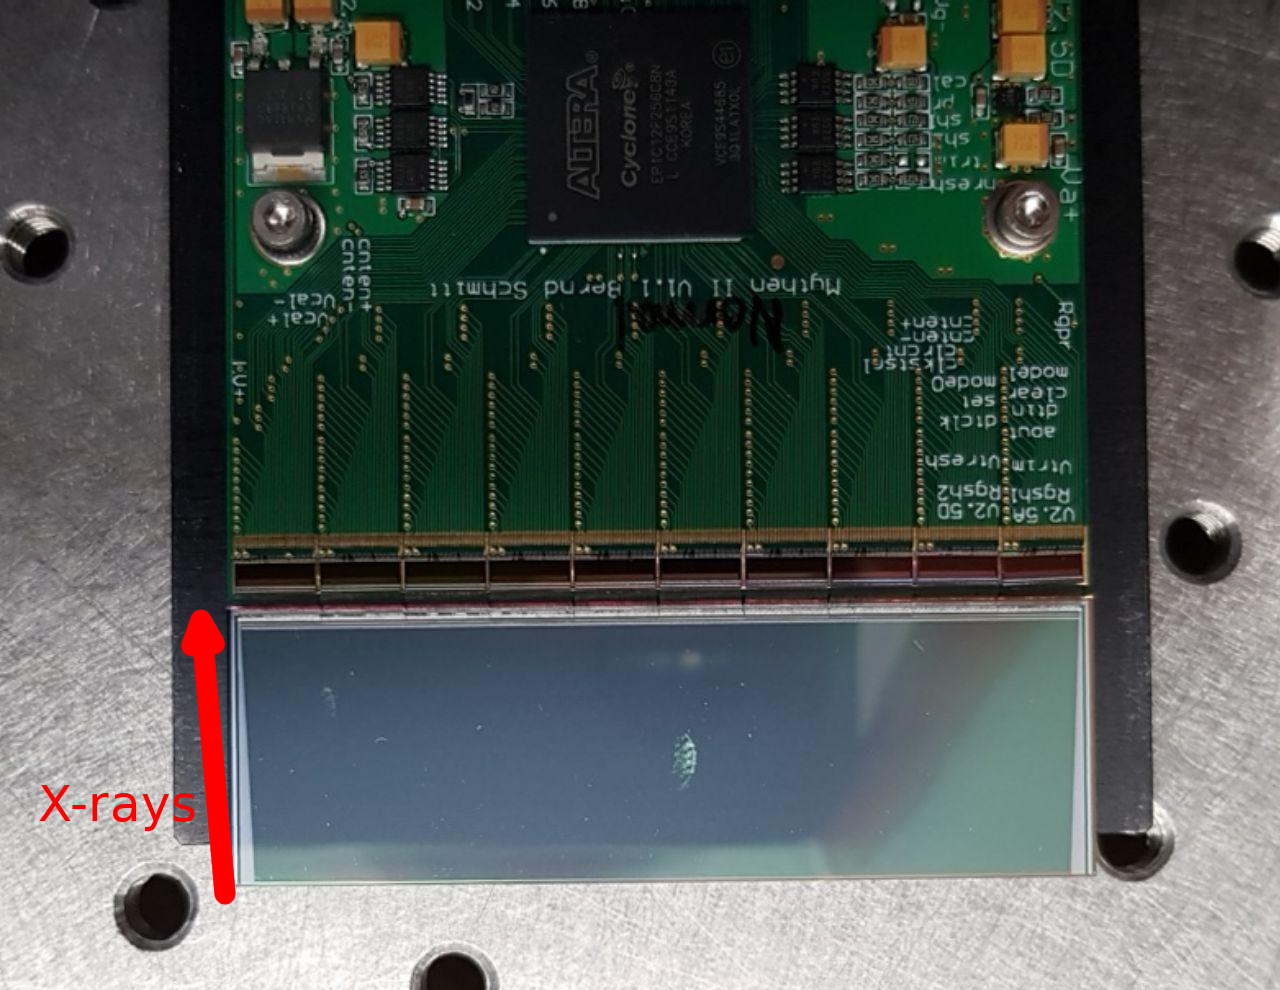
\includegraphics[width=\textwidth]{gfx/mythen-edge-on/mythen.png}
    \caption{}
    \end{subfigure}
    \begin{subfigure}[b]{.49\textwidth}
    \centering
    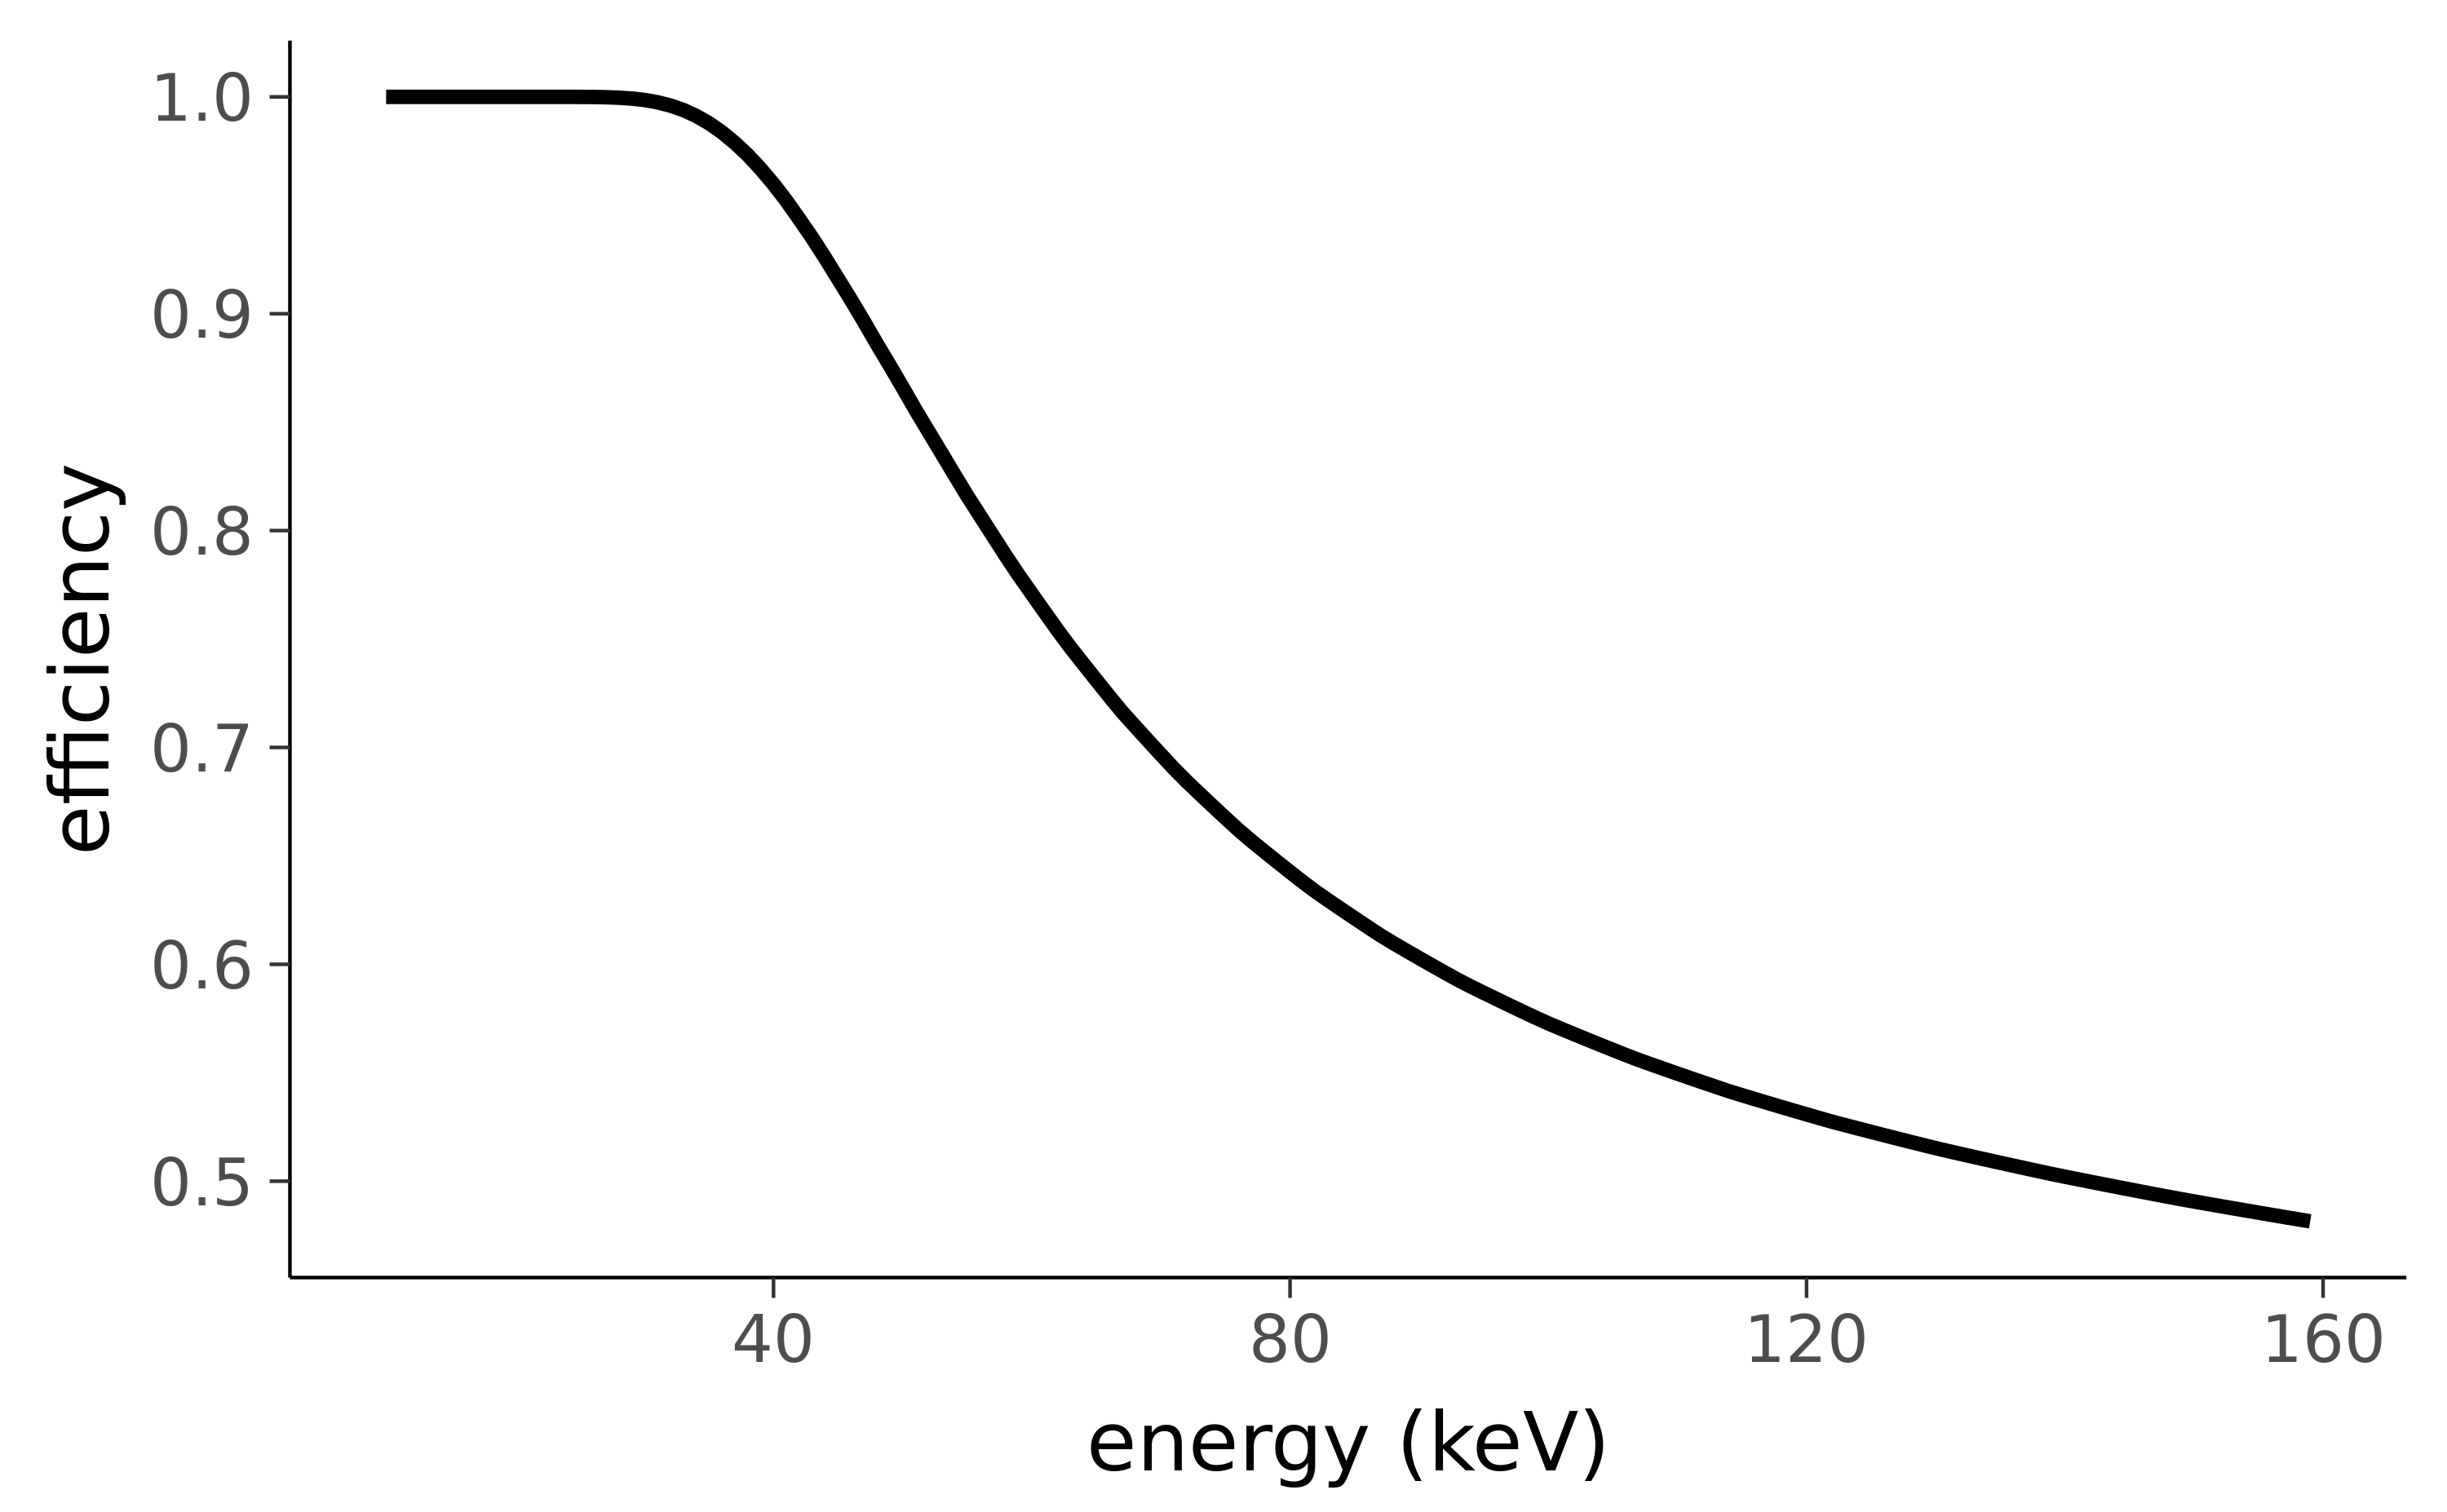
\includegraphics[width=\textwidth]{gfx/mythen-edge-on/efficiency.png}
    \caption{}
    \end{subfigure}
    \caption[Mythen detector module.]{A Mythen detector module~\parencite{SCHMITT2003267} with \SI{2}{\centi\meter} silicon
strips arranged to match a curved fan beam in the edge-on configuration.
This large thickness allows to reach a very high efficiency for a silicon
sensor, without compromising the resolution. The calculated efficiency is above
\SI{50}{\percent} up to \SI{160}{\kilo\eV}.}
    \label{fig:mythen-edge-on}
\end{figure}

The new custom made detector, matching the circular wave front, provides a
significant benefit for the visibility of the interference fringes, which is
improved from \SI{6}{\percent} (figures \ref{fig:visibility100}
and~\ref{fig:visibility120}) to an average of \SI{7.5}{\percent}, as shown in
figure~\ref{fig:mythen-visibility}.

\begin{figure}[htb]
    \centering
    \begin{subfigure}[b]{.49\textwidth}
    \centering
    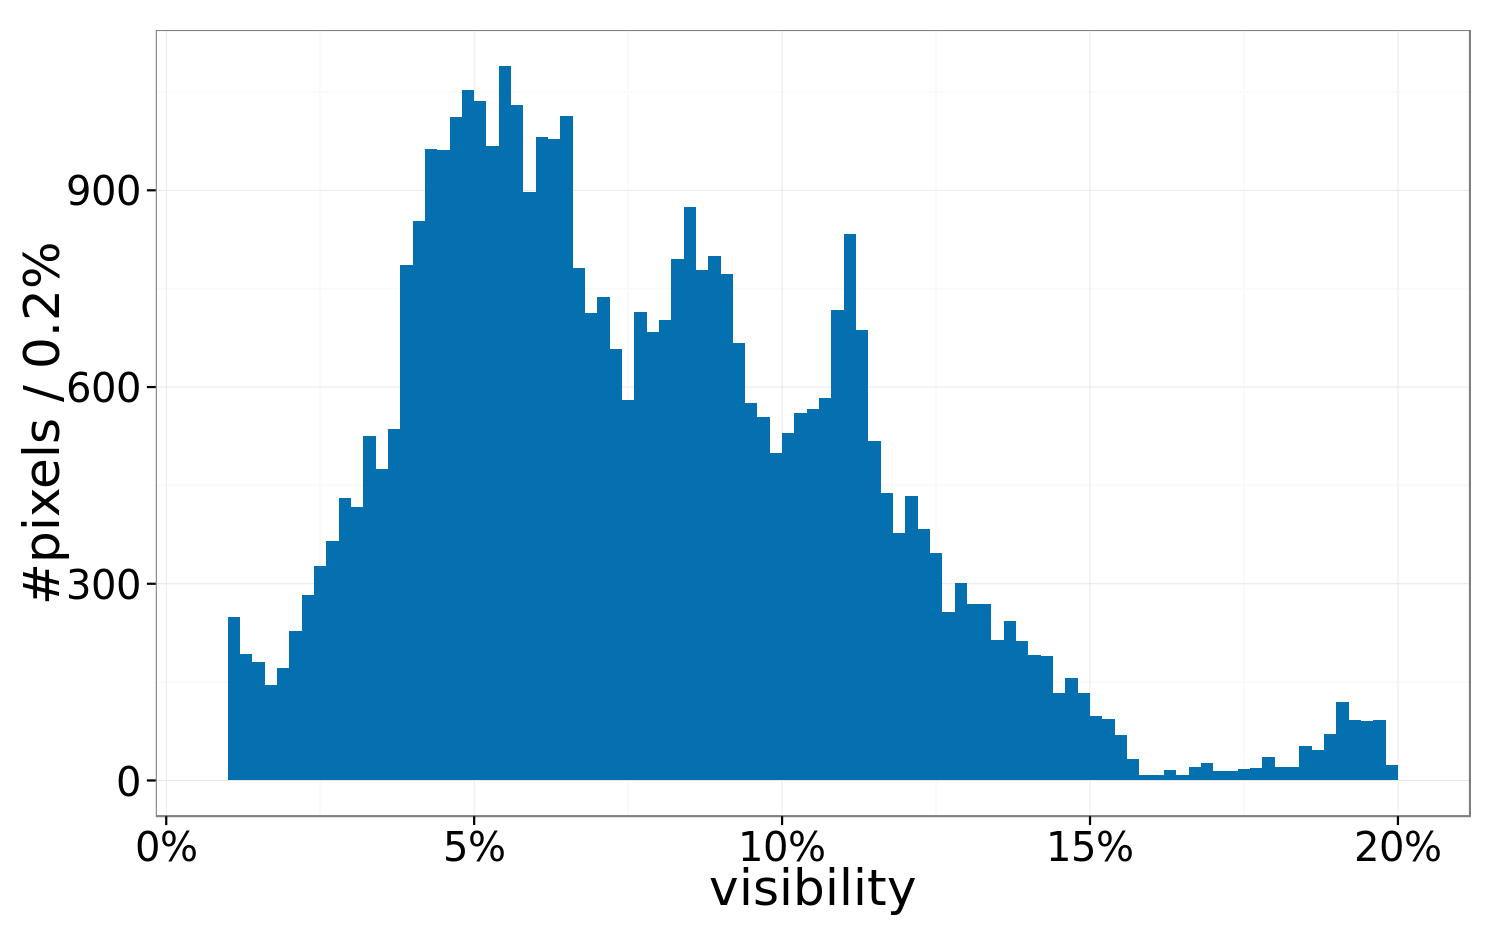
\includegraphics[width=\textwidth]{gfx/mythen-edge-on/visibility.png}
    \caption{}
    \label{fig:mythen-visibility}
    \end{subfigure}
    \hfill
    \begin{subfigure}[b]{.49\textwidth}
    \centering
    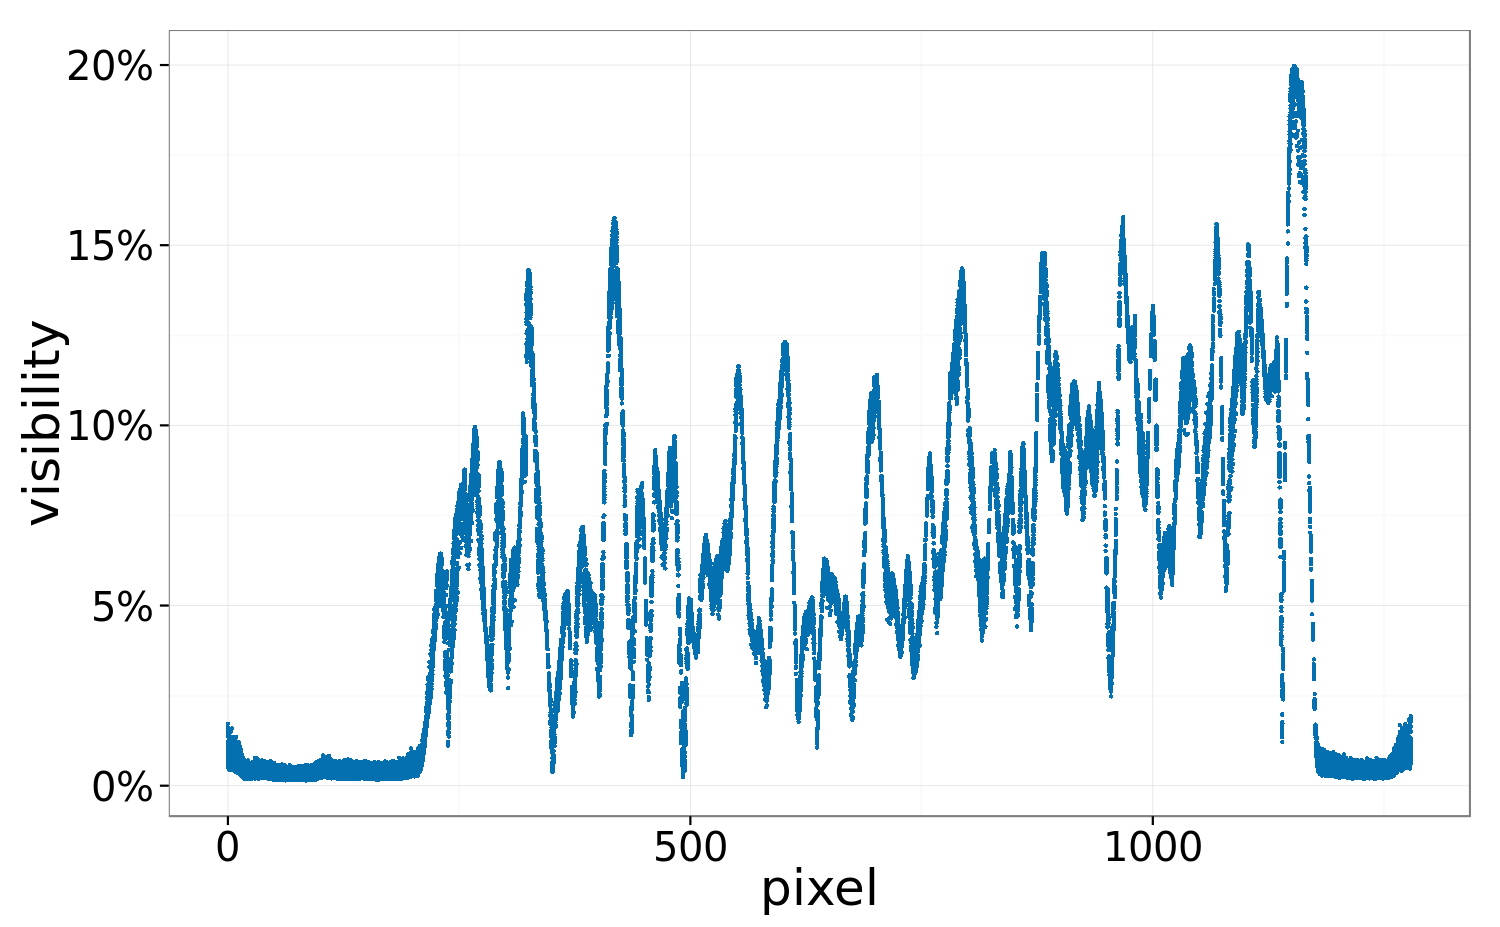
\includegraphics[width=\textwidth]{gfx/mythen-edge-on/pixel_visibility.png}
    \caption{}
    \label{fig:mythen-visibility-pixel}
    \end{subfigure}
    \caption[Visibility of the edge-on grating interferometer with a custom
    detector.]{Visibility histogram and visibility as a function of pixel
        number for the \SI{120}{\kilo\eV} design-energy interferometer with
        a custom silicon sensor matching the wave front curvature attached
        to a Mythen module~\parencite{SCHMITT2003267}.
    }
\end{figure}

\subsection{Phase drift for edge-on scans}
The edge-on grating arrangements allows the recording of a line at a time,
with a thickness of about \SI{50}{\micro\meter} at the sample position. This
means that a complete sample scan requires multiple line scans in order to
reconstruct a two-dimensional radiography.

It is a double scan procedure, as the phase stepping procedure is also
carried out to reconstruct the signals generated by the grating
interferometer. In practice, at each position $y$ of the sample, the grating
\G2 is stepped along $z$, after which the $z$ motor of the grating \G2 is
brought back at the starting position. The sample is then moved up along $y$
and a new phase stepping scan is started.

It was observed that this back-and-forth movement of the \G2 motor 
introduces a drift in the differential phase image: if the $z$ motor does
not come back to the exact starting position after each phase stepping scan,
the curve appears to be displaced even when no refraction is actually taking
place.

In order to observe this drift, many consecutive flat scans without sample are performed
and compared to the first scan. The result is shown in
figure~\ref{fig:phase.drift}. The phase differential phase has a constant
drift after each phase stepping scan, but it is possible to correct this
artifact with a simple linear fit. This correction was applied to all
datasets taken with the edge-on interferometer after reconstructing the differential
phase image.

\begin{figure}[htb]
    \centering
    \begin{subfigure}[b]{.75\textwidth}
        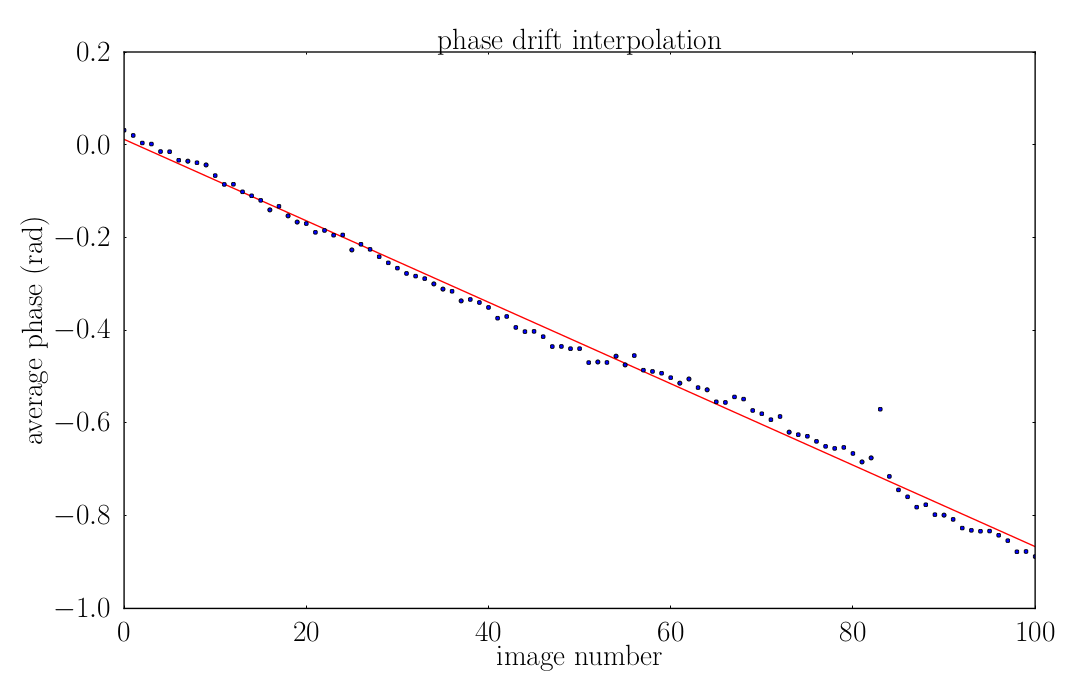
\includegraphics[width=\textwidth]{gfx/mythen-edge-on/drift_fit.png}
        \caption{}
    \end{subfigure}
    \begin{subfigure}[b]{.75\textwidth}
        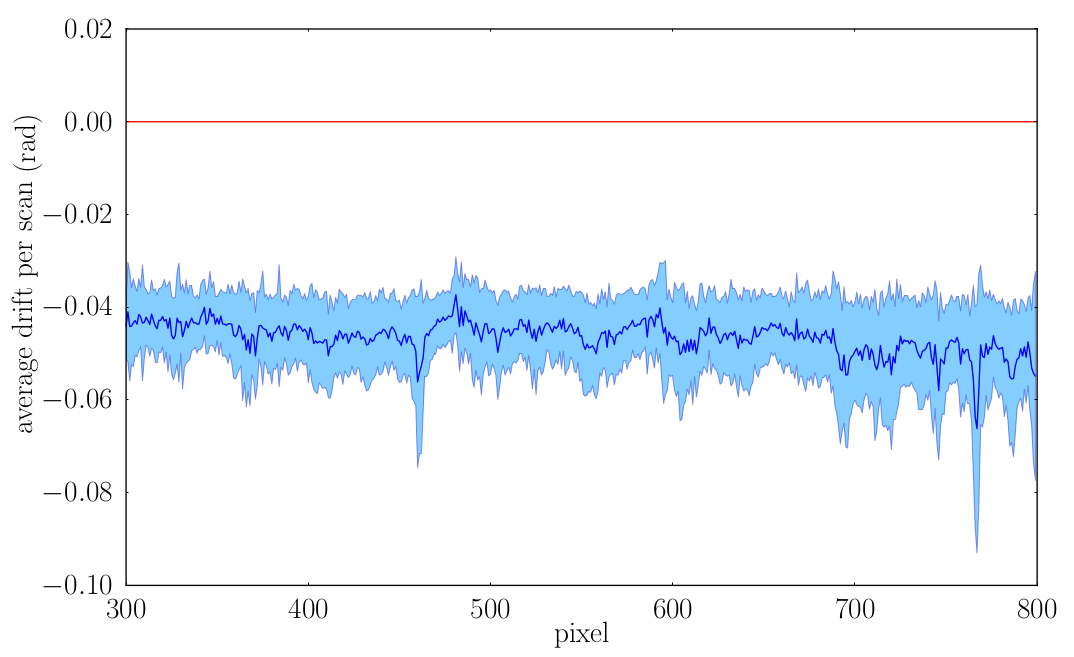
\includegraphics[width=\textwidth]{gfx/mythen-edge-on/drift_pixels.png}
        \caption{}
    \end{subfigure}
    \caption[Drift of the differential phase signal]{Drift of the differential phase signal for consecutive scans as
    a function of the number of scans (top), and on average as a function
of pixel (bottom). A linear correction can be applied, and it is
approximately constant across the whole field of view.}
    \label{fig:phase.drift}
\end{figure}

\subsection{Testing phase sensitivity}\label{sec:phase-sensitivity}
A quantitative test of the differential phase signal can be performed by
using samples in a shape of a wedge with an an angle $\theta$. Such a sample
introduces a constant deviation in the X-ray beam that can be measured and
then averaged across the whole field of view
(figure~\ref{fig:wedge.deviation}).

\begin{figure}[htb]
    \centering
    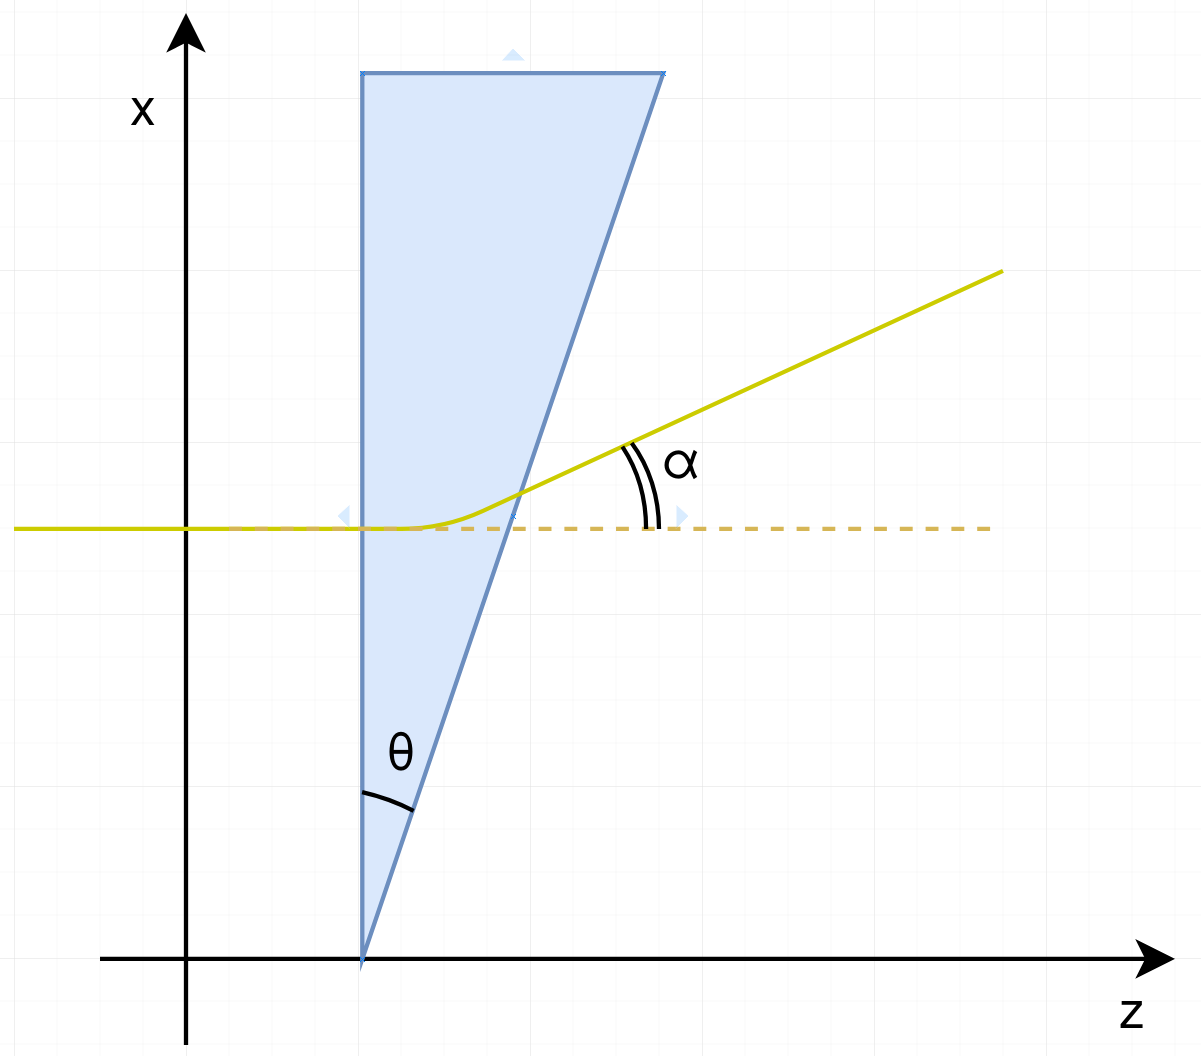
\includegraphics[width=.5\textwidth]{gfx/wedge-deviation.png}
    \caption{Deviation of X-rays introduced by a wedge sample with an angle
    $\theta$.}
    \label{fig:wedge.deviation}
\end{figure}

According to equation~\eqref{eq:phase.deviation}, a thickness $z$ of a
homogeneous material with refractive index $\delta$ introduces a change in
the phase of the X-ray beam according to $\phi = -k\delta z$. In the wedge,
the thickness $z$ depends on the position $x$ according to $z = x\tan
\theta$. Equation~\eqref{eq:differential.phase} shows that the grating
interferometer is not actually sensitive to $\phi$ but to its derivative
along the direction $x$, perpendicular to the grating lines. This is the
reason the wedge is an ideal shape for such measurements, since now the
relationship becomes simply
\begin{align}
    \alpha &= -\frac{1}{k}\partial_x\phi = \delta\tan\theta\\
    \delta &= \frac{2 \pi p_2 \tan \theta}{D_1}P,
    \label{eq:measuring.differential.phase}
\end{align}
where $P$ is the differential phase signal directly measured with the
interferometer. With this relationship between the real part of the
refractive index $\delta$ and the measured differential phase value $P$ we
can test our experiment by scanning three wedges made of plastic materials
and $\theta = \pi/6$: \ac{PMMA}, \ac{PS} and \ac{HDPE}.
The samples are scanned with an exposure time of \SI{5}{\second} for each of
the \num{9} phase steps.                 

The comparison with the expected values of $\delta$, taken at the average
energy of the spectrum (\SI{50}{\kilo\eV}), and the measured values shows a
good agreement (table~\ref{tab:delta.experiment})

\begin{table}[htb]
    \centering
    \begin{tabular}{*3c}
        \toprule
        material & $\delta_{\text{NIST}}$ ($\cdot 10^{-9})$ &
        $\delta_{\text{exp}}$ ($\cdot 10^{-9})$ \\
        \midrule
        PMMA & \num{102} & $92 \pm 19$\\
        PS & \num{90} & $81 \pm 21$\\
        HDPE & \num{88} & $87 \pm 14$\\
        \bottomrule
    \end{tabular}
    \caption{Comparison between values of the real part of the refractive
        index $\delta$ as measured with the \SI{120}{\kilo\eV} Talbot-Lau
        interferometer and taken from the NIST database~\parencite{nist}.}
    \label{tab:delta.experiment}
\end{table}

\subsection{Testing dark field sensitivity to microstructures}
It has been reported in many
studies~\parencite{Yashiro:10,Cong:12,Ritter:14,Schleede2012a,Meinel_2014,Scherer2015NoninvasiveDO}
that the dark field contrast arises whenever the sample contains very small
structures, on the scale of few
micrometers, that cannot be resolved by a detector pixel, but contribute to
decreasing the visibility of the interference pattern in a Talbot-Lau
interferometer.

In order to reproduce this phenomenon, rectangular plastic blocks filled
with different substances are scanned under different angles in the
interferometer. This allows to record images for different thicknesses of
the same material by only changing the rotation angle, with \num{9} phase
steps and \SI{5}{\second} exposure per step.

The images are segmented so that the region containing the material, that is
with the most absorption, is selected. More in detail, the minimum value in
the transmission profile is selected, and values up to
\SI{10}{\percent} higher than the minimum are kept.

The absorption and visibility reduction signals are used, according to the
definitions given in equations~\eqref{eq:visibility-definition}
and~\eqref{eq:dark-field-definition}.

\begin{align}
    A &= a_{0,s} / a_{0,f}\\
    B &= \frac{a_{1,s}}{a_{0,s}}\frac{a_{0,f}}{a_{1,f}}
    \label{eq:signal-definition-2}
\end{align}

The data are then averaged, and shown in figure~\ref{fig:powders} with $R =
\log(B) / \log(A)$ as a function of X-ray transmission, indicating different
thicknesses.

\begin{figure}[ht]
    \centering
    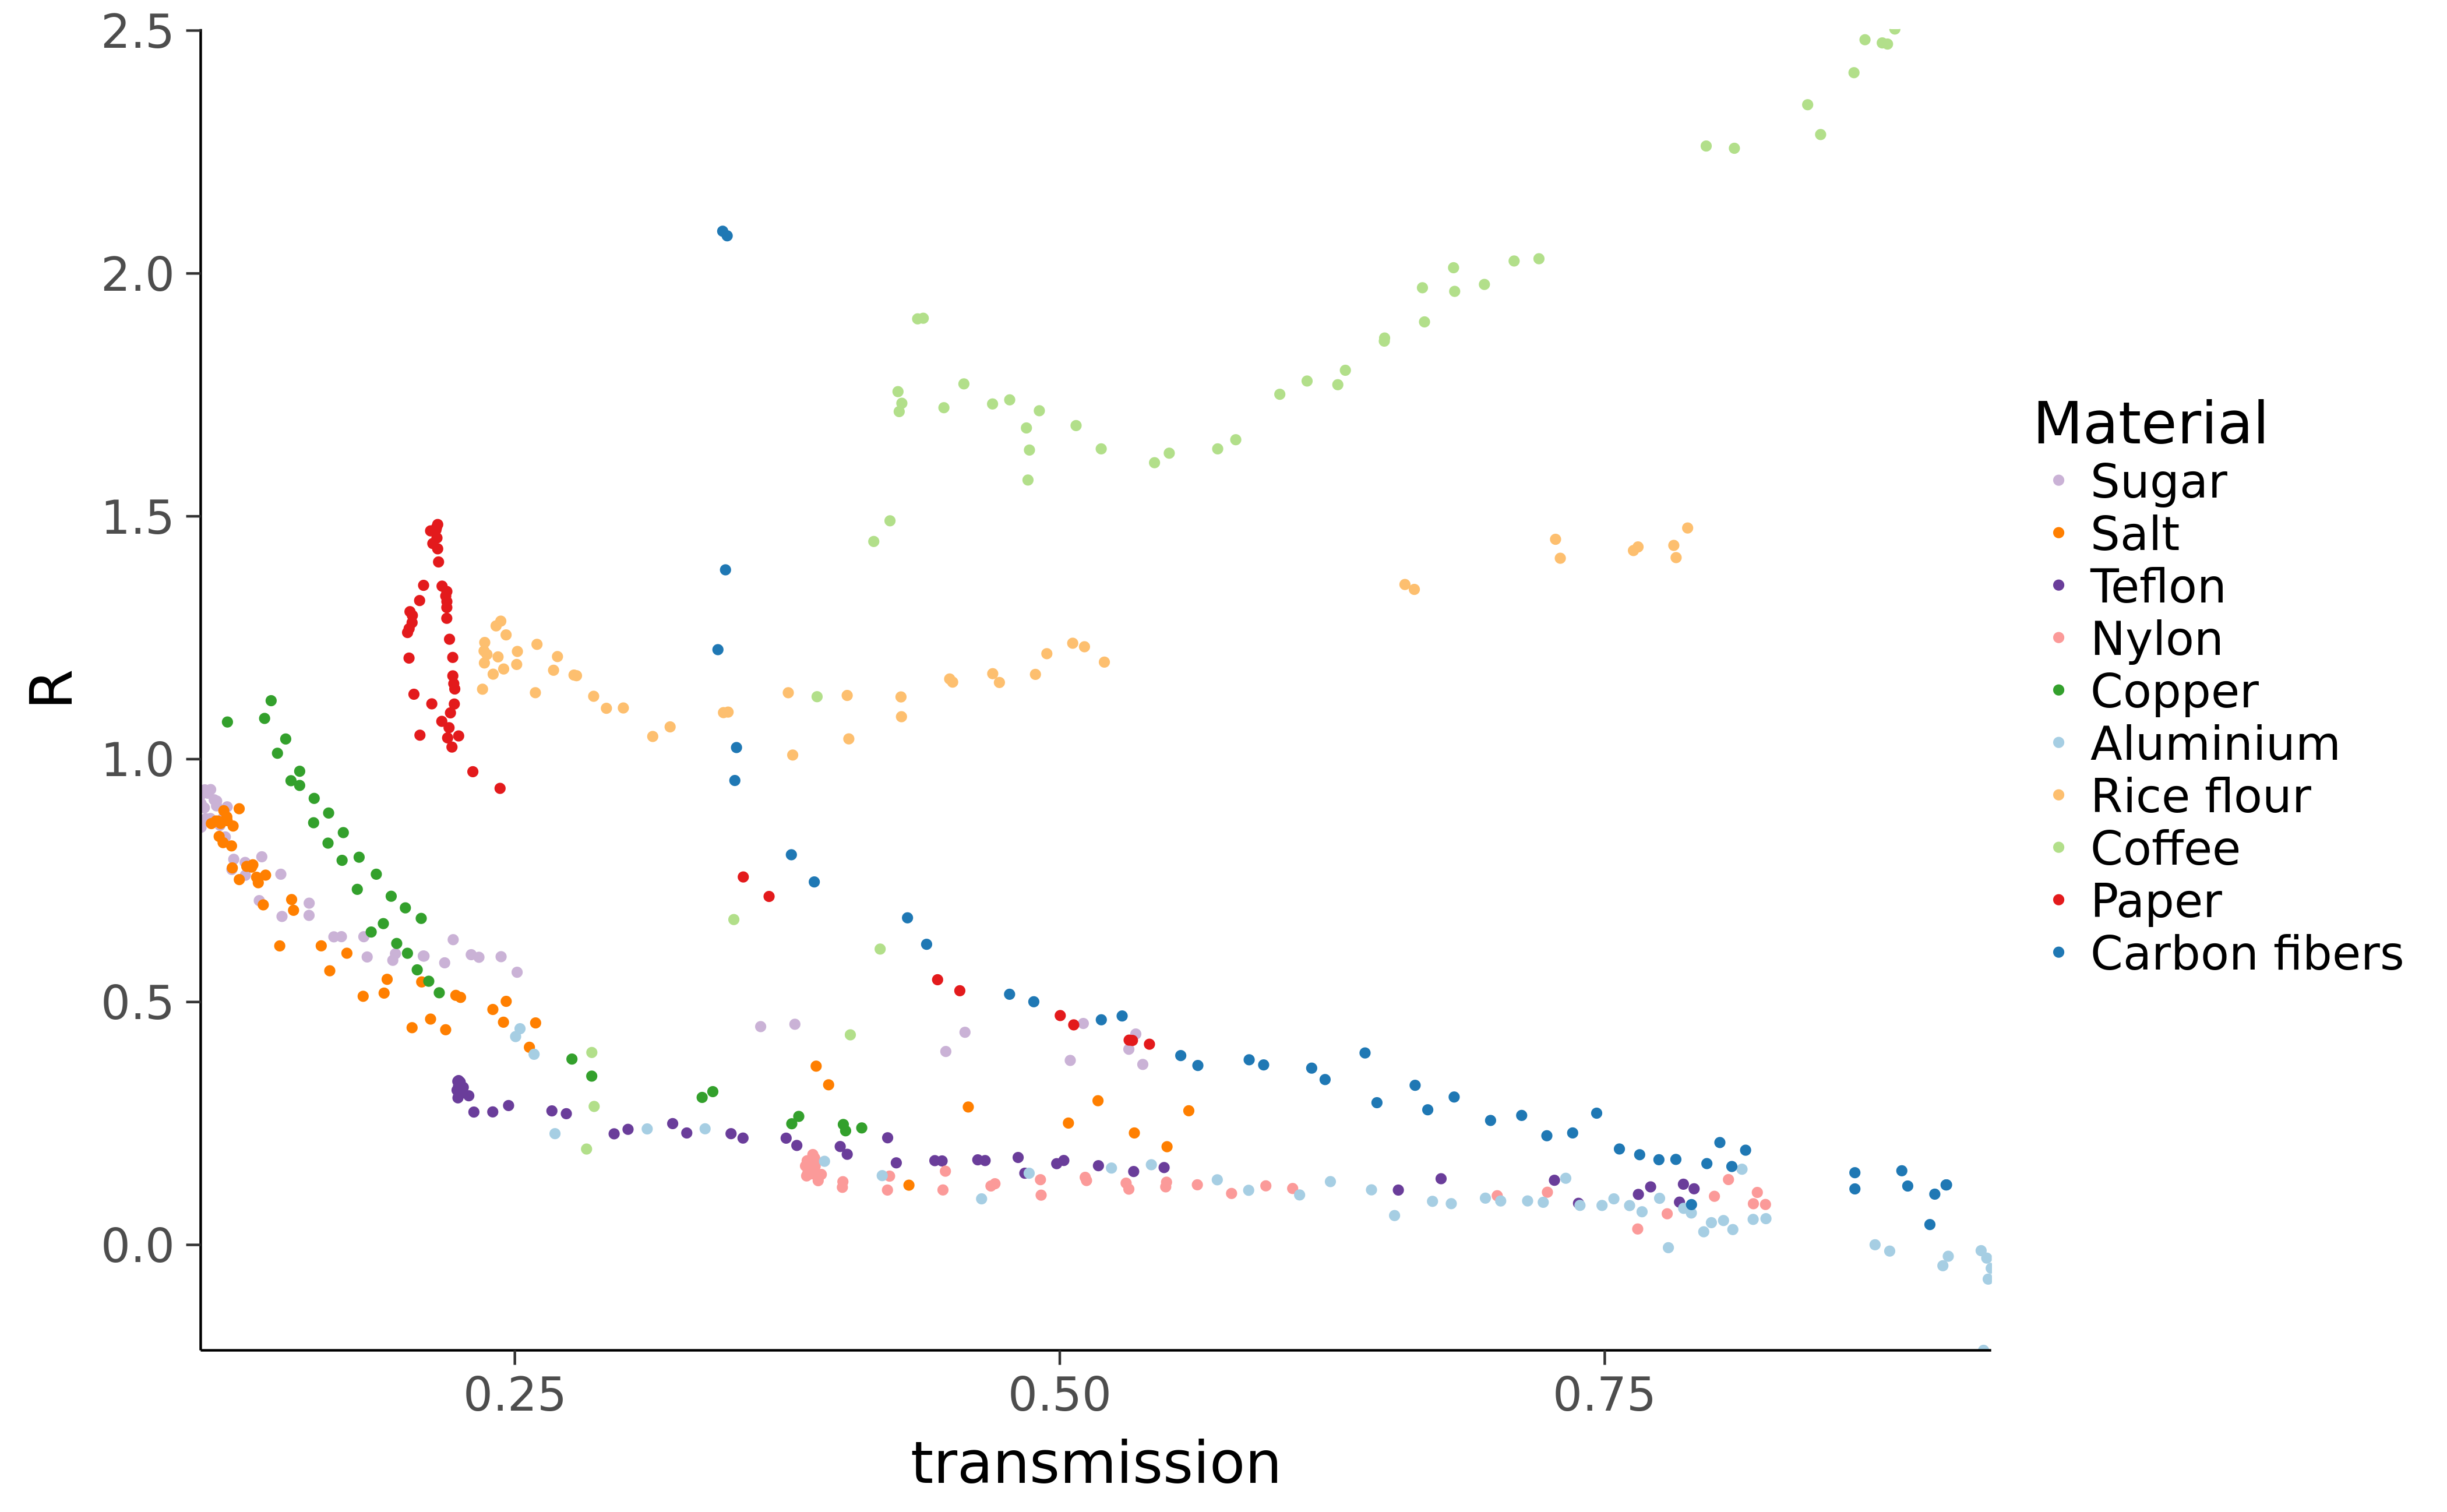
\includegraphics[width=\textwidth]{gfx/powders-aggregated.png}
    \caption{Ratio $R = \log(B) / \log(A)$ as a function of sample
    thickness, indicated by X-ray transmission, for different materials.}
    \label{fig:powders}
\end{figure}

Another interesting sample is a metal rod embedded in a polystyrene foam.
Foams are another class of samples that are particularly relevant for
dark-field imaging, providing enhanced contrast from the small air bubbles
in a matrix.

\begin{figure}[h!]
    \centering
    \begin{subfigure}[b]{.49\textwidth}
        \resizebox{\textwidth}{!}{\input{gfx/foam_sample.eepic}}
        \caption{}
    \end{subfigure}
    \begin{subfigure}[b]{.49\textwidth}
        \resizebox{\textwidth}{!}{%% Creator: Matplotlib, PGF backend
%%
%% To include the figure in your LaTeX document, write
%%   \input{<filename>.pgf}
%%
%% Make sure the required packages are loaded in your preamble
%%   \usepackage{pgf}
%%
%% Figures using additional raster images can only be included by \input if
%% they are in the same directory as the main LaTeX file. For loading figures
%% from other directories you can use the `import` package
%%   \usepackage{import}
%% and then include the figures with
%%   \import{<path to file>}{<filename>.pgf}
%%
%% Matplotlib used the following preamble
%%   \usepackage{fontspec}
%%
\begingroup%
\makeatletter%
\begin{pgfpicture}%
\pgfpathrectangle{\pgfpointorigin}{\pgfqpoint{4.600000in}{2.842800in}}%
\pgfusepath{use as bounding box, clip}%
\begin{pgfscope}%
\pgfsetbuttcap%
\pgfsetmiterjoin%
\definecolor{currentfill}{rgb}{1.000000,1.000000,1.000000}%
\pgfsetfillcolor{currentfill}%
\pgfsetlinewidth{0.000000pt}%
\definecolor{currentstroke}{rgb}{1.000000,1.000000,1.000000}%
\pgfsetstrokecolor{currentstroke}%
\pgfsetdash{}{0pt}%
\pgfpathmoveto{\pgfqpoint{0.000000in}{0.000000in}}%
\pgfpathlineto{\pgfqpoint{4.600000in}{0.000000in}}%
\pgfpathlineto{\pgfqpoint{4.600000in}{2.842800in}}%
\pgfpathlineto{\pgfqpoint{0.000000in}{2.842800in}}%
\pgfpathclose%
\pgfusepath{fill}%
\end{pgfscope}%
\begin{pgfscope}%
\pgfsetbuttcap%
\pgfsetmiterjoin%
\definecolor{currentfill}{rgb}{1.000000,1.000000,1.000000}%
\pgfsetfillcolor{currentfill}%
\pgfsetlinewidth{0.000000pt}%
\definecolor{currentstroke}{rgb}{0.000000,0.000000,0.000000}%
\pgfsetstrokecolor{currentstroke}%
\pgfsetstrokeopacity{0.000000}%
\pgfsetdash{}{0pt}%
\pgfpathmoveto{\pgfqpoint{0.575000in}{0.312708in}}%
\pgfpathlineto{\pgfqpoint{4.140000in}{0.312708in}}%
\pgfpathlineto{\pgfqpoint{4.140000in}{2.501664in}}%
\pgfpathlineto{\pgfqpoint{0.575000in}{2.501664in}}%
\pgfpathclose%
\pgfusepath{fill}%
\end{pgfscope}%
\begin{pgfscope}%
\pgfsetbuttcap%
\pgfsetroundjoin%
\definecolor{currentfill}{rgb}{0.000000,0.000000,0.000000}%
\pgfsetfillcolor{currentfill}%
\pgfsetlinewidth{0.803000pt}%
\definecolor{currentstroke}{rgb}{0.000000,0.000000,0.000000}%
\pgfsetstrokecolor{currentstroke}%
\pgfsetdash{}{0pt}%
\pgfsys@defobject{currentmarker}{\pgfqpoint{0.000000in}{-0.048611in}}{\pgfqpoint{0.000000in}{0.000000in}}{%
\pgfpathmoveto{\pgfqpoint{0.000000in}{0.000000in}}%
\pgfpathlineto{\pgfqpoint{0.000000in}{-0.048611in}}%
\pgfusepath{stroke,fill}%
}%
\begin{pgfscope}%
\pgfsys@transformshift{0.575000in}{0.312708in}%
\pgfsys@useobject{currentmarker}{}%
\end{pgfscope}%
\end{pgfscope}%
\begin{pgfscope}%
\pgftext[x=0.575000in,y=0.194652in,,top]{\rmfamily\fontsize{11.000000}{13.200000}\selectfont 0}%
\end{pgfscope}%
\begin{pgfscope}%
\pgfsetbuttcap%
\pgfsetroundjoin%
\definecolor{currentfill}{rgb}{0.000000,0.000000,0.000000}%
\pgfsetfillcolor{currentfill}%
\pgfsetlinewidth{0.803000pt}%
\definecolor{currentstroke}{rgb}{0.000000,0.000000,0.000000}%
\pgfsetstrokecolor{currentstroke}%
\pgfsetdash{}{0pt}%
\pgfsys@defobject{currentmarker}{\pgfqpoint{0.000000in}{-0.048611in}}{\pgfqpoint{0.000000in}{0.000000in}}{%
\pgfpathmoveto{\pgfqpoint{0.000000in}{0.000000in}}%
\pgfpathlineto{\pgfqpoint{0.000000in}{-0.048611in}}%
\pgfusepath{stroke,fill}%
}%
\begin{pgfscope}%
\pgfsys@transformshift{1.123462in}{0.312708in}%
\pgfsys@useobject{currentmarker}{}%
\end{pgfscope}%
\end{pgfscope}%
\begin{pgfscope}%
\pgftext[x=1.123462in,y=0.194652in,,top]{\rmfamily\fontsize{11.000000}{13.200000}\selectfont 100}%
\end{pgfscope}%
\begin{pgfscope}%
\pgfsetbuttcap%
\pgfsetroundjoin%
\definecolor{currentfill}{rgb}{0.000000,0.000000,0.000000}%
\pgfsetfillcolor{currentfill}%
\pgfsetlinewidth{0.803000pt}%
\definecolor{currentstroke}{rgb}{0.000000,0.000000,0.000000}%
\pgfsetstrokecolor{currentstroke}%
\pgfsetdash{}{0pt}%
\pgfsys@defobject{currentmarker}{\pgfqpoint{0.000000in}{-0.048611in}}{\pgfqpoint{0.000000in}{0.000000in}}{%
\pgfpathmoveto{\pgfqpoint{0.000000in}{0.000000in}}%
\pgfpathlineto{\pgfqpoint{0.000000in}{-0.048611in}}%
\pgfusepath{stroke,fill}%
}%
\begin{pgfscope}%
\pgfsys@transformshift{1.671923in}{0.312708in}%
\pgfsys@useobject{currentmarker}{}%
\end{pgfscope}%
\end{pgfscope}%
\begin{pgfscope}%
\pgftext[x=1.671923in,y=0.194652in,,top]{\rmfamily\fontsize{11.000000}{13.200000}\selectfont 200}%
\end{pgfscope}%
\begin{pgfscope}%
\pgfsetbuttcap%
\pgfsetroundjoin%
\definecolor{currentfill}{rgb}{0.000000,0.000000,0.000000}%
\pgfsetfillcolor{currentfill}%
\pgfsetlinewidth{0.803000pt}%
\definecolor{currentstroke}{rgb}{0.000000,0.000000,0.000000}%
\pgfsetstrokecolor{currentstroke}%
\pgfsetdash{}{0pt}%
\pgfsys@defobject{currentmarker}{\pgfqpoint{0.000000in}{-0.048611in}}{\pgfqpoint{0.000000in}{0.000000in}}{%
\pgfpathmoveto{\pgfqpoint{0.000000in}{0.000000in}}%
\pgfpathlineto{\pgfqpoint{0.000000in}{-0.048611in}}%
\pgfusepath{stroke,fill}%
}%
\begin{pgfscope}%
\pgfsys@transformshift{2.220385in}{0.312708in}%
\pgfsys@useobject{currentmarker}{}%
\end{pgfscope}%
\end{pgfscope}%
\begin{pgfscope}%
\pgftext[x=2.220385in,y=0.194652in,,top]{\rmfamily\fontsize{11.000000}{13.200000}\selectfont 300}%
\end{pgfscope}%
\begin{pgfscope}%
\pgfsetbuttcap%
\pgfsetroundjoin%
\definecolor{currentfill}{rgb}{0.000000,0.000000,0.000000}%
\pgfsetfillcolor{currentfill}%
\pgfsetlinewidth{0.803000pt}%
\definecolor{currentstroke}{rgb}{0.000000,0.000000,0.000000}%
\pgfsetstrokecolor{currentstroke}%
\pgfsetdash{}{0pt}%
\pgfsys@defobject{currentmarker}{\pgfqpoint{0.000000in}{-0.048611in}}{\pgfqpoint{0.000000in}{0.000000in}}{%
\pgfpathmoveto{\pgfqpoint{0.000000in}{0.000000in}}%
\pgfpathlineto{\pgfqpoint{0.000000in}{-0.048611in}}%
\pgfusepath{stroke,fill}%
}%
\begin{pgfscope}%
\pgfsys@transformshift{2.768846in}{0.312708in}%
\pgfsys@useobject{currentmarker}{}%
\end{pgfscope}%
\end{pgfscope}%
\begin{pgfscope}%
\pgftext[x=2.768846in,y=0.194652in,,top]{\rmfamily\fontsize{11.000000}{13.200000}\selectfont 400}%
\end{pgfscope}%
\begin{pgfscope}%
\pgfsetbuttcap%
\pgfsetroundjoin%
\definecolor{currentfill}{rgb}{0.000000,0.000000,0.000000}%
\pgfsetfillcolor{currentfill}%
\pgfsetlinewidth{0.803000pt}%
\definecolor{currentstroke}{rgb}{0.000000,0.000000,0.000000}%
\pgfsetstrokecolor{currentstroke}%
\pgfsetdash{}{0pt}%
\pgfsys@defobject{currentmarker}{\pgfqpoint{0.000000in}{-0.048611in}}{\pgfqpoint{0.000000in}{0.000000in}}{%
\pgfpathmoveto{\pgfqpoint{0.000000in}{0.000000in}}%
\pgfpathlineto{\pgfqpoint{0.000000in}{-0.048611in}}%
\pgfusepath{stroke,fill}%
}%
\begin{pgfscope}%
\pgfsys@transformshift{3.317308in}{0.312708in}%
\pgfsys@useobject{currentmarker}{}%
\end{pgfscope}%
\end{pgfscope}%
\begin{pgfscope}%
\pgftext[x=3.317308in,y=0.194652in,,top]{\rmfamily\fontsize{11.000000}{13.200000}\selectfont 500}%
\end{pgfscope}%
\begin{pgfscope}%
\pgfsetbuttcap%
\pgfsetroundjoin%
\definecolor{currentfill}{rgb}{0.000000,0.000000,0.000000}%
\pgfsetfillcolor{currentfill}%
\pgfsetlinewidth{0.803000pt}%
\definecolor{currentstroke}{rgb}{0.000000,0.000000,0.000000}%
\pgfsetstrokecolor{currentstroke}%
\pgfsetdash{}{0pt}%
\pgfsys@defobject{currentmarker}{\pgfqpoint{0.000000in}{-0.048611in}}{\pgfqpoint{0.000000in}{0.000000in}}{%
\pgfpathmoveto{\pgfqpoint{0.000000in}{0.000000in}}%
\pgfpathlineto{\pgfqpoint{0.000000in}{-0.048611in}}%
\pgfusepath{stroke,fill}%
}%
\begin{pgfscope}%
\pgfsys@transformshift{3.865769in}{0.312708in}%
\pgfsys@useobject{currentmarker}{}%
\end{pgfscope}%
\end{pgfscope}%
\begin{pgfscope}%
\pgftext[x=3.865769in,y=0.194652in,,top]{\rmfamily\fontsize{11.000000}{13.200000}\selectfont 600}%
\end{pgfscope}%
\begin{pgfscope}%
\pgftext[x=2.357500in,y=0.003430in,,top]{\rmfamily\fontsize{11.000000}{13.200000}\selectfont pixel}%
\end{pgfscope}%
\begin{pgfscope}%
\pgfsetbuttcap%
\pgfsetroundjoin%
\definecolor{currentfill}{rgb}{0.000000,0.000000,0.000000}%
\pgfsetfillcolor{currentfill}%
\pgfsetlinewidth{0.803000pt}%
\definecolor{currentstroke}{rgb}{0.000000,0.000000,0.000000}%
\pgfsetstrokecolor{currentstroke}%
\pgfsetdash{}{0pt}%
\pgfsys@defobject{currentmarker}{\pgfqpoint{-0.048611in}{0.000000in}}{\pgfqpoint{0.000000in}{0.000000in}}{%
\pgfpathmoveto{\pgfqpoint{0.000000in}{0.000000in}}%
\pgfpathlineto{\pgfqpoint{-0.048611in}{0.000000in}}%
\pgfusepath{stroke,fill}%
}%
\begin{pgfscope}%
\pgfsys@transformshift{0.575000in}{0.312708in}%
\pgfsys@useobject{currentmarker}{}%
\end{pgfscope}%
\end{pgfscope}%
\begin{pgfscope}%
\pgftext[x=0.265667in,y=0.259694in,left,base]{\rmfamily\fontsize{11.000000}{13.200000}\selectfont 0.0}%
\end{pgfscope}%
\begin{pgfscope}%
\pgfsetbuttcap%
\pgfsetroundjoin%
\definecolor{currentfill}{rgb}{0.000000,0.000000,0.000000}%
\pgfsetfillcolor{currentfill}%
\pgfsetlinewidth{0.803000pt}%
\definecolor{currentstroke}{rgb}{0.000000,0.000000,0.000000}%
\pgfsetstrokecolor{currentstroke}%
\pgfsetdash{}{0pt}%
\pgfsys@defobject{currentmarker}{\pgfqpoint{-0.048611in}{0.000000in}}{\pgfqpoint{0.000000in}{0.000000in}}{%
\pgfpathmoveto{\pgfqpoint{0.000000in}{0.000000in}}%
\pgfpathlineto{\pgfqpoint{-0.048611in}{0.000000in}}%
\pgfusepath{stroke,fill}%
}%
\begin{pgfscope}%
\pgfsys@transformshift{0.575000in}{0.710700in}%
\pgfsys@useobject{currentmarker}{}%
\end{pgfscope}%
\end{pgfscope}%
\begin{pgfscope}%
\pgftext[x=0.265667in,y=0.657686in,left,base]{\rmfamily\fontsize{11.000000}{13.200000}\selectfont 0.2}%
\end{pgfscope}%
\begin{pgfscope}%
\pgfsetbuttcap%
\pgfsetroundjoin%
\definecolor{currentfill}{rgb}{0.000000,0.000000,0.000000}%
\pgfsetfillcolor{currentfill}%
\pgfsetlinewidth{0.803000pt}%
\definecolor{currentstroke}{rgb}{0.000000,0.000000,0.000000}%
\pgfsetstrokecolor{currentstroke}%
\pgfsetdash{}{0pt}%
\pgfsys@defobject{currentmarker}{\pgfqpoint{-0.048611in}{0.000000in}}{\pgfqpoint{0.000000in}{0.000000in}}{%
\pgfpathmoveto{\pgfqpoint{0.000000in}{0.000000in}}%
\pgfpathlineto{\pgfqpoint{-0.048611in}{0.000000in}}%
\pgfusepath{stroke,fill}%
}%
\begin{pgfscope}%
\pgfsys@transformshift{0.575000in}{1.108692in}%
\pgfsys@useobject{currentmarker}{}%
\end{pgfscope}%
\end{pgfscope}%
\begin{pgfscope}%
\pgftext[x=0.265667in,y=1.055678in,left,base]{\rmfamily\fontsize{11.000000}{13.200000}\selectfont 0.4}%
\end{pgfscope}%
\begin{pgfscope}%
\pgfsetbuttcap%
\pgfsetroundjoin%
\definecolor{currentfill}{rgb}{0.000000,0.000000,0.000000}%
\pgfsetfillcolor{currentfill}%
\pgfsetlinewidth{0.803000pt}%
\definecolor{currentstroke}{rgb}{0.000000,0.000000,0.000000}%
\pgfsetstrokecolor{currentstroke}%
\pgfsetdash{}{0pt}%
\pgfsys@defobject{currentmarker}{\pgfqpoint{-0.048611in}{0.000000in}}{\pgfqpoint{0.000000in}{0.000000in}}{%
\pgfpathmoveto{\pgfqpoint{0.000000in}{0.000000in}}%
\pgfpathlineto{\pgfqpoint{-0.048611in}{0.000000in}}%
\pgfusepath{stroke,fill}%
}%
\begin{pgfscope}%
\pgfsys@transformshift{0.575000in}{1.506684in}%
\pgfsys@useobject{currentmarker}{}%
\end{pgfscope}%
\end{pgfscope}%
\begin{pgfscope}%
\pgftext[x=0.265667in,y=1.453670in,left,base]{\rmfamily\fontsize{11.000000}{13.200000}\selectfont 0.6}%
\end{pgfscope}%
\begin{pgfscope}%
\pgfsetbuttcap%
\pgfsetroundjoin%
\definecolor{currentfill}{rgb}{0.000000,0.000000,0.000000}%
\pgfsetfillcolor{currentfill}%
\pgfsetlinewidth{0.803000pt}%
\definecolor{currentstroke}{rgb}{0.000000,0.000000,0.000000}%
\pgfsetstrokecolor{currentstroke}%
\pgfsetdash{}{0pt}%
\pgfsys@defobject{currentmarker}{\pgfqpoint{-0.048611in}{0.000000in}}{\pgfqpoint{0.000000in}{0.000000in}}{%
\pgfpathmoveto{\pgfqpoint{0.000000in}{0.000000in}}%
\pgfpathlineto{\pgfqpoint{-0.048611in}{0.000000in}}%
\pgfusepath{stroke,fill}%
}%
\begin{pgfscope}%
\pgfsys@transformshift{0.575000in}{1.904676in}%
\pgfsys@useobject{currentmarker}{}%
\end{pgfscope}%
\end{pgfscope}%
\begin{pgfscope}%
\pgftext[x=0.265667in,y=1.851662in,left,base]{\rmfamily\fontsize{11.000000}{13.200000}\selectfont 0.8}%
\end{pgfscope}%
\begin{pgfscope}%
\pgfsetbuttcap%
\pgfsetroundjoin%
\definecolor{currentfill}{rgb}{0.000000,0.000000,0.000000}%
\pgfsetfillcolor{currentfill}%
\pgfsetlinewidth{0.803000pt}%
\definecolor{currentstroke}{rgb}{0.000000,0.000000,0.000000}%
\pgfsetstrokecolor{currentstroke}%
\pgfsetdash{}{0pt}%
\pgfsys@defobject{currentmarker}{\pgfqpoint{-0.048611in}{0.000000in}}{\pgfqpoint{0.000000in}{0.000000in}}{%
\pgfpathmoveto{\pgfqpoint{0.000000in}{0.000000in}}%
\pgfpathlineto{\pgfqpoint{-0.048611in}{0.000000in}}%
\pgfusepath{stroke,fill}%
}%
\begin{pgfscope}%
\pgfsys@transformshift{0.575000in}{2.302668in}%
\pgfsys@useobject{currentmarker}{}%
\end{pgfscope}%
\end{pgfscope}%
\begin{pgfscope}%
\pgftext[x=0.265667in,y=2.249654in,left,base]{\rmfamily\fontsize{11.000000}{13.200000}\selectfont 1.0}%
\end{pgfscope}%
\begin{pgfscope}%
\pgftext[x=0.210111in,y=1.407186in,,bottom,rotate=90.000000]{\rmfamily\fontsize{11.000000}{13.200000}\selectfont A, B}%
\end{pgfscope}%
\begin{pgfscope}%
\pgfpathrectangle{\pgfqpoint{0.575000in}{0.312708in}}{\pgfqpoint{3.565000in}{2.188956in}}%
\pgfusepath{clip}%
\pgfsetbuttcap%
\pgfsetroundjoin%
\pgfsetlinewidth{1.003750pt}%
\definecolor{currentstroke}{rgb}{0.000000,0.000000,0.000000}%
\pgfsetstrokecolor{currentstroke}%
\pgfsetdash{{3.700000pt}{1.600000pt}}{0.000000pt}%
\pgfpathmoveto{\pgfqpoint{0.575000in}{2.323902in}}%
\pgfpathlineto{\pgfqpoint{0.580485in}{2.325441in}}%
\pgfpathlineto{\pgfqpoint{0.591454in}{2.320174in}}%
\pgfpathlineto{\pgfqpoint{0.596938in}{2.320462in}}%
\pgfpathlineto{\pgfqpoint{0.602423in}{2.319613in}}%
\pgfpathlineto{\pgfqpoint{0.607908in}{2.325589in}}%
\pgfpathlineto{\pgfqpoint{0.613392in}{2.322660in}}%
\pgfpathlineto{\pgfqpoint{0.618877in}{2.325800in}}%
\pgfpathlineto{\pgfqpoint{0.624362in}{2.326491in}}%
\pgfpathlineto{\pgfqpoint{0.646300in}{2.320055in}}%
\pgfpathlineto{\pgfqpoint{0.651785in}{2.327083in}}%
\pgfpathlineto{\pgfqpoint{0.657269in}{2.319655in}}%
\pgfpathlineto{\pgfqpoint{0.662754in}{2.327252in}}%
\pgfpathlineto{\pgfqpoint{0.668238in}{2.323730in}}%
\pgfpathlineto{\pgfqpoint{0.679208in}{2.321071in}}%
\pgfpathlineto{\pgfqpoint{0.684692in}{2.321523in}}%
\pgfpathlineto{\pgfqpoint{0.695662in}{2.317139in}}%
\pgfpathlineto{\pgfqpoint{0.701146in}{2.317448in}}%
\pgfpathlineto{\pgfqpoint{0.706631in}{2.315147in}}%
\pgfpathlineto{\pgfqpoint{0.712115in}{2.321934in}}%
\pgfpathlineto{\pgfqpoint{0.717600in}{2.322123in}}%
\pgfpathlineto{\pgfqpoint{0.723085in}{2.328820in}}%
\pgfpathlineto{\pgfqpoint{0.728569in}{2.322202in}}%
\pgfpathlineto{\pgfqpoint{0.734054in}{2.322638in}}%
\pgfpathlineto{\pgfqpoint{0.739538in}{2.317752in}}%
\pgfpathlineto{\pgfqpoint{0.745023in}{2.317929in}}%
\pgfpathlineto{\pgfqpoint{0.750508in}{2.321071in}}%
\pgfpathlineto{\pgfqpoint{0.755992in}{2.320920in}}%
\pgfpathlineto{\pgfqpoint{0.761477in}{2.316986in}}%
\pgfpathlineto{\pgfqpoint{0.766962in}{2.320577in}}%
\pgfpathlineto{\pgfqpoint{0.772446in}{2.322204in}}%
\pgfpathlineto{\pgfqpoint{0.788900in}{2.316541in}}%
\pgfpathlineto{\pgfqpoint{0.799869in}{2.323419in}}%
\pgfpathlineto{\pgfqpoint{0.805354in}{2.317570in}}%
\pgfpathlineto{\pgfqpoint{0.816323in}{2.322590in}}%
\pgfpathlineto{\pgfqpoint{0.821808in}{2.317005in}}%
\pgfpathlineto{\pgfqpoint{0.827292in}{2.319489in}}%
\pgfpathlineto{\pgfqpoint{0.832777in}{2.323339in}}%
\pgfpathlineto{\pgfqpoint{0.838262in}{2.319088in}}%
\pgfpathlineto{\pgfqpoint{0.843746in}{2.322924in}}%
\pgfpathlineto{\pgfqpoint{0.849231in}{2.322660in}}%
\pgfpathlineto{\pgfqpoint{0.854715in}{2.320835in}}%
\pgfpathlineto{\pgfqpoint{0.860200in}{2.324342in}}%
\pgfpathlineto{\pgfqpoint{0.865685in}{2.323336in}}%
\pgfpathlineto{\pgfqpoint{0.871169in}{2.324136in}}%
\pgfpathlineto{\pgfqpoint{0.876654in}{2.322641in}}%
\pgfpathlineto{\pgfqpoint{0.893108in}{2.325304in}}%
\pgfpathlineto{\pgfqpoint{0.898592in}{2.324683in}}%
\pgfpathlineto{\pgfqpoint{0.904077in}{2.319775in}}%
\pgfpathlineto{\pgfqpoint{0.909562in}{2.319481in}}%
\pgfpathlineto{\pgfqpoint{0.915046in}{2.322041in}}%
\pgfpathlineto{\pgfqpoint{0.926015in}{2.320282in}}%
\pgfpathlineto{\pgfqpoint{0.931500in}{2.317624in}}%
\pgfpathlineto{\pgfqpoint{0.936985in}{2.323869in}}%
\pgfpathlineto{\pgfqpoint{0.942469in}{2.323755in}}%
\pgfpathlineto{\pgfqpoint{0.947954in}{2.317887in}}%
\pgfpathlineto{\pgfqpoint{0.953438in}{2.319807in}}%
\pgfpathlineto{\pgfqpoint{0.958923in}{2.324011in}}%
\pgfpathlineto{\pgfqpoint{0.964408in}{2.324286in}}%
\pgfpathlineto{\pgfqpoint{0.969892in}{2.319626in}}%
\pgfpathlineto{\pgfqpoint{0.975377in}{2.321185in}}%
\pgfpathlineto{\pgfqpoint{0.980862in}{2.320605in}}%
\pgfpathlineto{\pgfqpoint{0.986346in}{2.323638in}}%
\pgfpathlineto{\pgfqpoint{0.991831in}{2.319729in}}%
\pgfpathlineto{\pgfqpoint{1.002800in}{2.320011in}}%
\pgfpathlineto{\pgfqpoint{1.013769in}{2.318652in}}%
\pgfpathlineto{\pgfqpoint{1.019254in}{2.321210in}}%
\pgfpathlineto{\pgfqpoint{1.024738in}{2.319893in}}%
\pgfpathlineto{\pgfqpoint{1.030223in}{2.323702in}}%
\pgfpathlineto{\pgfqpoint{1.041192in}{2.320577in}}%
\pgfpathlineto{\pgfqpoint{1.046677in}{2.325169in}}%
\pgfpathlineto{\pgfqpoint{1.057646in}{2.322026in}}%
\pgfpathlineto{\pgfqpoint{1.074100in}{2.323506in}}%
\pgfpathlineto{\pgfqpoint{1.085069in}{2.316341in}}%
\pgfpathlineto{\pgfqpoint{1.090554in}{2.320516in}}%
\pgfpathlineto{\pgfqpoint{1.096038in}{2.322613in}}%
\pgfpathlineto{\pgfqpoint{1.101523in}{2.320006in}}%
\pgfpathlineto{\pgfqpoint{1.107008in}{2.320696in}}%
\pgfpathlineto{\pgfqpoint{1.112492in}{2.322714in}}%
\pgfpathlineto{\pgfqpoint{1.117977in}{2.319136in}}%
\pgfpathlineto{\pgfqpoint{1.123462in}{2.324167in}}%
\pgfpathlineto{\pgfqpoint{1.128946in}{2.320139in}}%
\pgfpathlineto{\pgfqpoint{1.139915in}{2.322677in}}%
\pgfpathlineto{\pgfqpoint{1.145400in}{2.320469in}}%
\pgfpathlineto{\pgfqpoint{1.156369in}{2.322773in}}%
\pgfpathlineto{\pgfqpoint{1.161854in}{2.323545in}}%
\pgfpathlineto{\pgfqpoint{1.167338in}{2.321364in}}%
\pgfpathlineto{\pgfqpoint{1.172823in}{2.320634in}}%
\pgfpathlineto{\pgfqpoint{1.178308in}{2.322297in}}%
\pgfpathlineto{\pgfqpoint{1.189277in}{2.318797in}}%
\pgfpathlineto{\pgfqpoint{1.194762in}{2.320047in}}%
\pgfpathlineto{\pgfqpoint{1.200246in}{2.324639in}}%
\pgfpathlineto{\pgfqpoint{1.216700in}{2.322166in}}%
\pgfpathlineto{\pgfqpoint{1.222185in}{2.324385in}}%
\pgfpathlineto{\pgfqpoint{1.233154in}{2.322909in}}%
\pgfpathlineto{\pgfqpoint{1.238638in}{2.325822in}}%
\pgfpathlineto{\pgfqpoint{1.244123in}{2.324430in}}%
\pgfpathlineto{\pgfqpoint{1.249608in}{2.325970in}}%
\pgfpathlineto{\pgfqpoint{1.255092in}{2.325938in}}%
\pgfpathlineto{\pgfqpoint{1.266062in}{2.329401in}}%
\pgfpathlineto{\pgfqpoint{1.271546in}{2.326500in}}%
\pgfpathlineto{\pgfqpoint{1.277031in}{2.327713in}}%
\pgfpathlineto{\pgfqpoint{1.282515in}{2.326993in}}%
\pgfpathlineto{\pgfqpoint{1.288000in}{2.328558in}}%
\pgfpathlineto{\pgfqpoint{1.293485in}{2.327104in}}%
\pgfpathlineto{\pgfqpoint{1.304454in}{2.321193in}}%
\pgfpathlineto{\pgfqpoint{1.309938in}{2.324815in}}%
\pgfpathlineto{\pgfqpoint{1.315423in}{2.325247in}}%
\pgfpathlineto{\pgfqpoint{1.320908in}{2.323358in}}%
\pgfpathlineto{\pgfqpoint{1.326392in}{2.324293in}}%
\pgfpathlineto{\pgfqpoint{1.331877in}{2.322751in}}%
\pgfpathlineto{\pgfqpoint{1.342846in}{2.328202in}}%
\pgfpathlineto{\pgfqpoint{1.353815in}{2.322380in}}%
\pgfpathlineto{\pgfqpoint{1.364785in}{2.326716in}}%
\pgfpathlineto{\pgfqpoint{1.370269in}{2.328029in}}%
\pgfpathlineto{\pgfqpoint{1.375754in}{2.324391in}}%
\pgfpathlineto{\pgfqpoint{1.381238in}{2.324886in}}%
\pgfpathlineto{\pgfqpoint{1.386723in}{2.322668in}}%
\pgfpathlineto{\pgfqpoint{1.392208in}{2.328234in}}%
\pgfpathlineto{\pgfqpoint{1.397692in}{2.321590in}}%
\pgfpathlineto{\pgfqpoint{1.403177in}{2.322968in}}%
\pgfpathlineto{\pgfqpoint{1.408662in}{2.325744in}}%
\pgfpathlineto{\pgfqpoint{1.414146in}{2.323426in}}%
\pgfpathlineto{\pgfqpoint{1.419631in}{2.323122in}}%
\pgfpathlineto{\pgfqpoint{1.425115in}{2.325716in}}%
\pgfpathlineto{\pgfqpoint{1.430600in}{2.324212in}}%
\pgfpathlineto{\pgfqpoint{1.436085in}{2.327165in}}%
\pgfpathlineto{\pgfqpoint{1.447054in}{2.323585in}}%
\pgfpathlineto{\pgfqpoint{1.452538in}{2.321110in}}%
\pgfpathlineto{\pgfqpoint{1.458023in}{2.320944in}}%
\pgfpathlineto{\pgfqpoint{1.474477in}{2.326362in}}%
\pgfpathlineto{\pgfqpoint{1.479962in}{2.325332in}}%
\pgfpathlineto{\pgfqpoint{1.485446in}{2.326061in}}%
\pgfpathlineto{\pgfqpoint{1.490931in}{2.322367in}}%
\pgfpathlineto{\pgfqpoint{1.496415in}{2.325171in}}%
\pgfpathlineto{\pgfqpoint{1.501900in}{2.324537in}}%
\pgfpathlineto{\pgfqpoint{1.518354in}{2.318440in}}%
\pgfpathlineto{\pgfqpoint{1.523838in}{2.320698in}}%
\pgfpathlineto{\pgfqpoint{1.529323in}{2.318201in}}%
\pgfpathlineto{\pgfqpoint{1.551262in}{2.302155in}}%
\pgfpathlineto{\pgfqpoint{1.556746in}{2.296969in}}%
\pgfpathlineto{\pgfqpoint{1.562231in}{2.300293in}}%
\pgfpathlineto{\pgfqpoint{1.573200in}{2.290880in}}%
\pgfpathlineto{\pgfqpoint{1.578685in}{2.288046in}}%
\pgfpathlineto{\pgfqpoint{1.584169in}{2.287670in}}%
\pgfpathlineto{\pgfqpoint{1.595138in}{2.283412in}}%
\pgfpathlineto{\pgfqpoint{1.600623in}{2.285110in}}%
\pgfpathlineto{\pgfqpoint{1.611592in}{2.284145in}}%
\pgfpathlineto{\pgfqpoint{1.617077in}{2.280935in}}%
\pgfpathlineto{\pgfqpoint{1.628046in}{2.283289in}}%
\pgfpathlineto{\pgfqpoint{1.633531in}{2.279090in}}%
\pgfpathlineto{\pgfqpoint{1.639015in}{2.282563in}}%
\pgfpathlineto{\pgfqpoint{1.644500in}{2.287392in}}%
\pgfpathlineto{\pgfqpoint{1.649985in}{2.285565in}}%
\pgfpathlineto{\pgfqpoint{1.655469in}{2.285897in}}%
\pgfpathlineto{\pgfqpoint{1.660954in}{2.288308in}}%
\pgfpathlineto{\pgfqpoint{1.666438in}{2.285857in}}%
\pgfpathlineto{\pgfqpoint{1.671923in}{2.285889in}}%
\pgfpathlineto{\pgfqpoint{1.677408in}{2.287961in}}%
\pgfpathlineto{\pgfqpoint{1.682892in}{2.277056in}}%
\pgfpathlineto{\pgfqpoint{1.688377in}{2.280972in}}%
\pgfpathlineto{\pgfqpoint{1.693862in}{2.278640in}}%
\pgfpathlineto{\pgfqpoint{1.699346in}{2.280011in}}%
\pgfpathlineto{\pgfqpoint{1.704831in}{2.278363in}}%
\pgfpathlineto{\pgfqpoint{1.710315in}{2.278838in}}%
\pgfpathlineto{\pgfqpoint{1.715800in}{2.278007in}}%
\pgfpathlineto{\pgfqpoint{1.721285in}{2.280419in}}%
\pgfpathlineto{\pgfqpoint{1.726769in}{2.284523in}}%
\pgfpathlineto{\pgfqpoint{1.732254in}{2.279617in}}%
\pgfpathlineto{\pgfqpoint{1.737738in}{2.277276in}}%
\pgfpathlineto{\pgfqpoint{1.748708in}{2.282368in}}%
\pgfpathlineto{\pgfqpoint{1.754192in}{2.277018in}}%
\pgfpathlineto{\pgfqpoint{1.759677in}{2.278081in}}%
\pgfpathlineto{\pgfqpoint{1.770646in}{2.278518in}}%
\pgfpathlineto{\pgfqpoint{1.776131in}{2.273877in}}%
\pgfpathlineto{\pgfqpoint{1.781615in}{2.271784in}}%
\pgfpathlineto{\pgfqpoint{1.787100in}{2.274257in}}%
\pgfpathlineto{\pgfqpoint{1.792585in}{2.270696in}}%
\pgfpathlineto{\pgfqpoint{1.798069in}{2.275737in}}%
\pgfpathlineto{\pgfqpoint{1.809038in}{2.272560in}}%
\pgfpathlineto{\pgfqpoint{1.814523in}{2.272545in}}%
\pgfpathlineto{\pgfqpoint{1.820008in}{2.275389in}}%
\pgfpathlineto{\pgfqpoint{1.825492in}{2.271969in}}%
\pgfpathlineto{\pgfqpoint{1.830977in}{2.271750in}}%
\pgfpathlineto{\pgfqpoint{1.841946in}{2.279598in}}%
\pgfpathlineto{\pgfqpoint{1.847431in}{2.278214in}}%
\pgfpathlineto{\pgfqpoint{1.852915in}{2.274754in}}%
\pgfpathlineto{\pgfqpoint{1.858400in}{2.278109in}}%
\pgfpathlineto{\pgfqpoint{1.863885in}{2.282989in}}%
\pgfpathlineto{\pgfqpoint{1.869369in}{2.276352in}}%
\pgfpathlineto{\pgfqpoint{1.874854in}{2.277894in}}%
\pgfpathlineto{\pgfqpoint{1.880338in}{2.272748in}}%
\pgfpathlineto{\pgfqpoint{1.885823in}{2.272926in}}%
\pgfpathlineto{\pgfqpoint{1.896792in}{2.270867in}}%
\pgfpathlineto{\pgfqpoint{1.907762in}{2.276128in}}%
\pgfpathlineto{\pgfqpoint{1.913246in}{2.275337in}}%
\pgfpathlineto{\pgfqpoint{1.918731in}{2.279451in}}%
\pgfpathlineto{\pgfqpoint{1.924215in}{2.273961in}}%
\pgfpathlineto{\pgfqpoint{1.929700in}{2.279134in}}%
\pgfpathlineto{\pgfqpoint{1.935185in}{2.279782in}}%
\pgfpathlineto{\pgfqpoint{1.940669in}{2.277522in}}%
\pgfpathlineto{\pgfqpoint{1.946154in}{2.282481in}}%
\pgfpathlineto{\pgfqpoint{1.951638in}{2.276230in}}%
\pgfpathlineto{\pgfqpoint{1.957123in}{2.281794in}}%
\pgfpathlineto{\pgfqpoint{1.968092in}{2.277718in}}%
\pgfpathlineto{\pgfqpoint{1.973577in}{2.284544in}}%
\pgfpathlineto{\pgfqpoint{1.979062in}{2.279214in}}%
\pgfpathlineto{\pgfqpoint{1.984546in}{2.290918in}}%
\pgfpathlineto{\pgfqpoint{1.990031in}{2.279283in}}%
\pgfpathlineto{\pgfqpoint{1.995515in}{2.278846in}}%
\pgfpathlineto{\pgfqpoint{2.006485in}{2.281293in}}%
\pgfpathlineto{\pgfqpoint{2.011969in}{2.279620in}}%
\pgfpathlineto{\pgfqpoint{2.017454in}{2.284135in}}%
\pgfpathlineto{\pgfqpoint{2.022938in}{2.284093in}}%
\pgfpathlineto{\pgfqpoint{2.028423in}{2.282404in}}%
\pgfpathlineto{\pgfqpoint{2.033908in}{2.281985in}}%
\pgfpathlineto{\pgfqpoint{2.039392in}{2.279594in}}%
\pgfpathlineto{\pgfqpoint{2.050362in}{2.265875in}}%
\pgfpathlineto{\pgfqpoint{2.055846in}{2.260758in}}%
\pgfpathlineto{\pgfqpoint{2.061331in}{2.252207in}}%
\pgfpathlineto{\pgfqpoint{2.066815in}{2.233206in}}%
\pgfpathlineto{\pgfqpoint{2.077785in}{2.174359in}}%
\pgfpathlineto{\pgfqpoint{2.088754in}{2.080783in}}%
\pgfpathlineto{\pgfqpoint{2.094238in}{2.025053in}}%
\pgfpathlineto{\pgfqpoint{2.105208in}{1.884705in}}%
\pgfpathlineto{\pgfqpoint{2.127146in}{1.556046in}}%
\pgfpathlineto{\pgfqpoint{2.138115in}{1.430232in}}%
\pgfpathlineto{\pgfqpoint{2.149085in}{1.335225in}}%
\pgfpathlineto{\pgfqpoint{2.160054in}{1.270773in}}%
\pgfpathlineto{\pgfqpoint{2.176508in}{1.204376in}}%
\pgfpathlineto{\pgfqpoint{2.187477in}{1.177019in}}%
\pgfpathlineto{\pgfqpoint{2.192962in}{1.168650in}}%
\pgfpathlineto{\pgfqpoint{2.198446in}{1.156762in}}%
\pgfpathlineto{\pgfqpoint{2.203931in}{1.150982in}}%
\pgfpathlineto{\pgfqpoint{2.214900in}{1.136527in}}%
\pgfpathlineto{\pgfqpoint{2.220385in}{1.133459in}}%
\pgfpathlineto{\pgfqpoint{2.225869in}{1.126720in}}%
\pgfpathlineto{\pgfqpoint{2.231354in}{1.123283in}}%
\pgfpathlineto{\pgfqpoint{2.253292in}{1.116857in}}%
\pgfpathlineto{\pgfqpoint{2.258777in}{1.117284in}}%
\pgfpathlineto{\pgfqpoint{2.264262in}{1.114914in}}%
\pgfpathlineto{\pgfqpoint{2.269746in}{1.114318in}}%
\pgfpathlineto{\pgfqpoint{2.275231in}{1.116686in}}%
\pgfpathlineto{\pgfqpoint{2.291685in}{1.135011in}}%
\pgfpathlineto{\pgfqpoint{2.297169in}{1.142827in}}%
\pgfpathlineto{\pgfqpoint{2.319108in}{1.184851in}}%
\pgfpathlineto{\pgfqpoint{2.330077in}{1.217371in}}%
\pgfpathlineto{\pgfqpoint{2.335562in}{1.234937in}}%
\pgfpathlineto{\pgfqpoint{2.346531in}{1.283198in}}%
\pgfpathlineto{\pgfqpoint{2.352015in}{1.314959in}}%
\pgfpathlineto{\pgfqpoint{2.362985in}{1.394769in}}%
\pgfpathlineto{\pgfqpoint{2.373954in}{1.504716in}}%
\pgfpathlineto{\pgfqpoint{2.384923in}{1.637488in}}%
\pgfpathlineto{\pgfqpoint{2.417831in}{2.093541in}}%
\pgfpathlineto{\pgfqpoint{2.428800in}{2.186813in}}%
\pgfpathlineto{\pgfqpoint{2.434285in}{2.212476in}}%
\pgfpathlineto{\pgfqpoint{2.439769in}{2.231491in}}%
\pgfpathlineto{\pgfqpoint{2.450738in}{2.258664in}}%
\pgfpathlineto{\pgfqpoint{2.456223in}{2.263131in}}%
\pgfpathlineto{\pgfqpoint{2.461708in}{2.272295in}}%
\pgfpathlineto{\pgfqpoint{2.467192in}{2.269825in}}%
\pgfpathlineto{\pgfqpoint{2.478162in}{2.273873in}}%
\pgfpathlineto{\pgfqpoint{2.489131in}{2.271223in}}%
\pgfpathlineto{\pgfqpoint{2.500100in}{2.274880in}}%
\pgfpathlineto{\pgfqpoint{2.505585in}{2.269590in}}%
\pgfpathlineto{\pgfqpoint{2.516554in}{2.272527in}}%
\pgfpathlineto{\pgfqpoint{2.522038in}{2.276590in}}%
\pgfpathlineto{\pgfqpoint{2.527523in}{2.277755in}}%
\pgfpathlineto{\pgfqpoint{2.533008in}{2.277639in}}%
\pgfpathlineto{\pgfqpoint{2.538492in}{2.275480in}}%
\pgfpathlineto{\pgfqpoint{2.543977in}{2.274646in}}%
\pgfpathlineto{\pgfqpoint{2.554946in}{2.282488in}}%
\pgfpathlineto{\pgfqpoint{2.560431in}{2.279111in}}%
\pgfpathlineto{\pgfqpoint{2.565915in}{2.282851in}}%
\pgfpathlineto{\pgfqpoint{2.576885in}{2.279190in}}%
\pgfpathlineto{\pgfqpoint{2.582369in}{2.282767in}}%
\pgfpathlineto{\pgfqpoint{2.593338in}{2.281137in}}%
\pgfpathlineto{\pgfqpoint{2.604308in}{2.276067in}}%
\pgfpathlineto{\pgfqpoint{2.609792in}{2.280417in}}%
\pgfpathlineto{\pgfqpoint{2.615277in}{2.277363in}}%
\pgfpathlineto{\pgfqpoint{2.620762in}{2.275975in}}%
\pgfpathlineto{\pgfqpoint{2.626246in}{2.276057in}}%
\pgfpathlineto{\pgfqpoint{2.631731in}{2.274189in}}%
\pgfpathlineto{\pgfqpoint{2.637215in}{2.270648in}}%
\pgfpathlineto{\pgfqpoint{2.642700in}{2.278163in}}%
\pgfpathlineto{\pgfqpoint{2.648185in}{2.274245in}}%
\pgfpathlineto{\pgfqpoint{2.653669in}{2.272238in}}%
\pgfpathlineto{\pgfqpoint{2.659154in}{2.275329in}}%
\pgfpathlineto{\pgfqpoint{2.670123in}{2.276901in}}%
\pgfpathlineto{\pgfqpoint{2.675608in}{2.280985in}}%
\pgfpathlineto{\pgfqpoint{2.681092in}{2.280653in}}%
\pgfpathlineto{\pgfqpoint{2.686577in}{2.273487in}}%
\pgfpathlineto{\pgfqpoint{2.692062in}{2.278767in}}%
\pgfpathlineto{\pgfqpoint{2.697546in}{2.272837in}}%
\pgfpathlineto{\pgfqpoint{2.703031in}{2.271215in}}%
\pgfpathlineto{\pgfqpoint{2.708515in}{2.273409in}}%
\pgfpathlineto{\pgfqpoint{2.714000in}{2.277009in}}%
\pgfpathlineto{\pgfqpoint{2.719485in}{2.275564in}}%
\pgfpathlineto{\pgfqpoint{2.724969in}{2.280046in}}%
\pgfpathlineto{\pgfqpoint{2.730454in}{2.278406in}}%
\pgfpathlineto{\pgfqpoint{2.735938in}{2.280186in}}%
\pgfpathlineto{\pgfqpoint{2.741423in}{2.278082in}}%
\pgfpathlineto{\pgfqpoint{2.746908in}{2.284145in}}%
\pgfpathlineto{\pgfqpoint{2.752392in}{2.280151in}}%
\pgfpathlineto{\pgfqpoint{2.757877in}{2.282195in}}%
\pgfpathlineto{\pgfqpoint{2.763362in}{2.278855in}}%
\pgfpathlineto{\pgfqpoint{2.768846in}{2.277585in}}%
\pgfpathlineto{\pgfqpoint{2.774331in}{2.285666in}}%
\pgfpathlineto{\pgfqpoint{2.779815in}{2.281900in}}%
\pgfpathlineto{\pgfqpoint{2.785300in}{2.284816in}}%
\pgfpathlineto{\pgfqpoint{2.790785in}{2.278562in}}%
\pgfpathlineto{\pgfqpoint{2.807238in}{2.280061in}}%
\pgfpathlineto{\pgfqpoint{2.812723in}{2.286677in}}%
\pgfpathlineto{\pgfqpoint{2.818208in}{2.281996in}}%
\pgfpathlineto{\pgfqpoint{2.823692in}{2.285167in}}%
\pgfpathlineto{\pgfqpoint{2.834662in}{2.286475in}}%
\pgfpathlineto{\pgfqpoint{2.840146in}{2.281591in}}%
\pgfpathlineto{\pgfqpoint{2.845631in}{2.281841in}}%
\pgfpathlineto{\pgfqpoint{2.851115in}{2.287631in}}%
\pgfpathlineto{\pgfqpoint{2.856600in}{2.279996in}}%
\pgfpathlineto{\pgfqpoint{2.862085in}{2.284950in}}%
\pgfpathlineto{\pgfqpoint{2.878538in}{2.284141in}}%
\pgfpathlineto{\pgfqpoint{2.884023in}{2.287412in}}%
\pgfpathlineto{\pgfqpoint{2.889508in}{2.284889in}}%
\pgfpathlineto{\pgfqpoint{2.900477in}{2.286327in}}%
\pgfpathlineto{\pgfqpoint{2.911446in}{2.277655in}}%
\pgfpathlineto{\pgfqpoint{2.916931in}{2.286541in}}%
\pgfpathlineto{\pgfqpoint{2.922415in}{2.287331in}}%
\pgfpathlineto{\pgfqpoint{2.927900in}{2.285032in}}%
\pgfpathlineto{\pgfqpoint{2.933385in}{2.286739in}}%
\pgfpathlineto{\pgfqpoint{2.938869in}{2.283071in}}%
\pgfpathlineto{\pgfqpoint{2.944354in}{2.287446in}}%
\pgfpathlineto{\pgfqpoint{2.949838in}{2.285866in}}%
\pgfpathlineto{\pgfqpoint{2.960808in}{2.285062in}}%
\pgfpathlineto{\pgfqpoint{2.966292in}{2.288195in}}%
\pgfpathlineto{\pgfqpoint{2.971777in}{2.288252in}}%
\pgfpathlineto{\pgfqpoint{2.977262in}{2.286667in}}%
\pgfpathlineto{\pgfqpoint{2.982746in}{2.286939in}}%
\pgfpathlineto{\pgfqpoint{2.993715in}{2.284015in}}%
\pgfpathlineto{\pgfqpoint{3.004685in}{2.284495in}}%
\pgfpathlineto{\pgfqpoint{3.010169in}{2.288005in}}%
\pgfpathlineto{\pgfqpoint{3.015654in}{2.285930in}}%
\pgfpathlineto{\pgfqpoint{3.021138in}{2.282549in}}%
\pgfpathlineto{\pgfqpoint{3.026623in}{2.282550in}}%
\pgfpathlineto{\pgfqpoint{3.032108in}{2.285228in}}%
\pgfpathlineto{\pgfqpoint{3.048562in}{2.285528in}}%
\pgfpathlineto{\pgfqpoint{3.054046in}{2.290677in}}%
\pgfpathlineto{\pgfqpoint{3.059531in}{2.286382in}}%
\pgfpathlineto{\pgfqpoint{3.075985in}{2.288827in}}%
\pgfpathlineto{\pgfqpoint{3.081469in}{2.288569in}}%
\pgfpathlineto{\pgfqpoint{3.086954in}{2.291976in}}%
\pgfpathlineto{\pgfqpoint{3.092438in}{2.292291in}}%
\pgfpathlineto{\pgfqpoint{3.097923in}{2.294572in}}%
\pgfpathlineto{\pgfqpoint{3.103408in}{2.290862in}}%
\pgfpathlineto{\pgfqpoint{3.119862in}{2.295614in}}%
\pgfpathlineto{\pgfqpoint{3.125346in}{2.293848in}}%
\pgfpathlineto{\pgfqpoint{3.130831in}{2.296032in}}%
\pgfpathlineto{\pgfqpoint{3.136315in}{2.300704in}}%
\pgfpathlineto{\pgfqpoint{3.141800in}{2.297067in}}%
\pgfpathlineto{\pgfqpoint{3.147285in}{2.296992in}}%
\pgfpathlineto{\pgfqpoint{3.152769in}{2.299508in}}%
\pgfpathlineto{\pgfqpoint{3.163738in}{2.309784in}}%
\pgfpathlineto{\pgfqpoint{3.169223in}{2.305663in}}%
\pgfpathlineto{\pgfqpoint{3.174708in}{2.309006in}}%
\pgfpathlineto{\pgfqpoint{3.180192in}{2.309398in}}%
\pgfpathlineto{\pgfqpoint{3.185677in}{2.306053in}}%
\pgfpathlineto{\pgfqpoint{3.191162in}{2.311772in}}%
\pgfpathlineto{\pgfqpoint{3.196646in}{2.308514in}}%
\pgfpathlineto{\pgfqpoint{3.213100in}{2.312112in}}%
\pgfpathlineto{\pgfqpoint{3.218585in}{2.309644in}}%
\pgfpathlineto{\pgfqpoint{3.224069in}{2.312394in}}%
\pgfpathlineto{\pgfqpoint{3.229554in}{2.311466in}}%
\pgfpathlineto{\pgfqpoint{3.235038in}{2.313370in}}%
\pgfpathlineto{\pgfqpoint{3.240523in}{2.310705in}}%
\pgfpathlineto{\pgfqpoint{3.246008in}{2.313955in}}%
\pgfpathlineto{\pgfqpoint{3.251492in}{2.309230in}}%
\pgfpathlineto{\pgfqpoint{3.256977in}{2.312404in}}%
\pgfpathlineto{\pgfqpoint{3.262462in}{2.309976in}}%
\pgfpathlineto{\pgfqpoint{3.273431in}{2.313304in}}%
\pgfpathlineto{\pgfqpoint{3.278915in}{2.310999in}}%
\pgfpathlineto{\pgfqpoint{3.284400in}{2.315065in}}%
\pgfpathlineto{\pgfqpoint{3.289885in}{2.316425in}}%
\pgfpathlineto{\pgfqpoint{3.300854in}{2.314142in}}%
\pgfpathlineto{\pgfqpoint{3.306338in}{2.316770in}}%
\pgfpathlineto{\pgfqpoint{3.311823in}{2.310215in}}%
\pgfpathlineto{\pgfqpoint{3.322792in}{2.318799in}}%
\pgfpathlineto{\pgfqpoint{3.328277in}{2.320244in}}%
\pgfpathlineto{\pgfqpoint{3.333762in}{2.315595in}}%
\pgfpathlineto{\pgfqpoint{3.339246in}{2.323573in}}%
\pgfpathlineto{\pgfqpoint{3.344731in}{2.317989in}}%
\pgfpathlineto{\pgfqpoint{3.350215in}{2.320915in}}%
\pgfpathlineto{\pgfqpoint{3.355700in}{2.315960in}}%
\pgfpathlineto{\pgfqpoint{3.361185in}{2.315532in}}%
\pgfpathlineto{\pgfqpoint{3.366669in}{2.320318in}}%
\pgfpathlineto{\pgfqpoint{3.372154in}{2.321894in}}%
\pgfpathlineto{\pgfqpoint{3.377638in}{2.319398in}}%
\pgfpathlineto{\pgfqpoint{3.383123in}{2.320777in}}%
\pgfpathlineto{\pgfqpoint{3.388608in}{2.325410in}}%
\pgfpathlineto{\pgfqpoint{3.394092in}{2.323436in}}%
\pgfpathlineto{\pgfqpoint{3.399577in}{2.326518in}}%
\pgfpathlineto{\pgfqpoint{3.405062in}{2.327836in}}%
\pgfpathlineto{\pgfqpoint{3.421515in}{2.323598in}}%
\pgfpathlineto{\pgfqpoint{3.427000in}{2.325063in}}%
\pgfpathlineto{\pgfqpoint{3.432485in}{2.329734in}}%
\pgfpathlineto{\pgfqpoint{3.443454in}{2.329559in}}%
\pgfpathlineto{\pgfqpoint{3.454423in}{2.325373in}}%
\pgfpathlineto{\pgfqpoint{3.459908in}{2.328614in}}%
\pgfpathlineto{\pgfqpoint{3.465392in}{2.327917in}}%
\pgfpathlineto{\pgfqpoint{3.470877in}{2.328409in}}%
\pgfpathlineto{\pgfqpoint{3.476362in}{2.323577in}}%
\pgfpathlineto{\pgfqpoint{3.481846in}{2.328910in}}%
\pgfpathlineto{\pgfqpoint{3.487331in}{2.329872in}}%
\pgfpathlineto{\pgfqpoint{3.492815in}{2.325212in}}%
\pgfpathlineto{\pgfqpoint{3.498300in}{2.331488in}}%
\pgfpathlineto{\pgfqpoint{3.503785in}{2.325991in}}%
\pgfpathlineto{\pgfqpoint{3.509269in}{2.327429in}}%
\pgfpathlineto{\pgfqpoint{3.514754in}{2.330325in}}%
\pgfpathlineto{\pgfqpoint{3.520238in}{2.326112in}}%
\pgfpathlineto{\pgfqpoint{3.531208in}{2.327108in}}%
\pgfpathlineto{\pgfqpoint{3.536692in}{2.325744in}}%
\pgfpathlineto{\pgfqpoint{3.542177in}{2.327247in}}%
\pgfpathlineto{\pgfqpoint{3.553146in}{2.326654in}}%
\pgfpathlineto{\pgfqpoint{3.558631in}{2.324899in}}%
\pgfpathlineto{\pgfqpoint{3.564115in}{2.327020in}}%
\pgfpathlineto{\pgfqpoint{3.569600in}{2.327409in}}%
\pgfpathlineto{\pgfqpoint{3.575085in}{2.329403in}}%
\pgfpathlineto{\pgfqpoint{3.580569in}{2.328153in}}%
\pgfpathlineto{\pgfqpoint{3.586054in}{2.328861in}}%
\pgfpathlineto{\pgfqpoint{3.591538in}{2.331150in}}%
\pgfpathlineto{\pgfqpoint{3.597023in}{2.326772in}}%
\pgfpathlineto{\pgfqpoint{3.602508in}{2.333854in}}%
\pgfpathlineto{\pgfqpoint{3.607992in}{2.327695in}}%
\pgfpathlineto{\pgfqpoint{3.613477in}{2.331321in}}%
\pgfpathlineto{\pgfqpoint{3.618962in}{2.331411in}}%
\pgfpathlineto{\pgfqpoint{3.624446in}{2.327319in}}%
\pgfpathlineto{\pgfqpoint{3.629931in}{2.329985in}}%
\pgfpathlineto{\pgfqpoint{3.635415in}{2.327853in}}%
\pgfpathlineto{\pgfqpoint{3.640900in}{2.323582in}}%
\pgfpathlineto{\pgfqpoint{3.657354in}{2.329205in}}%
\pgfpathlineto{\pgfqpoint{3.662838in}{2.326746in}}%
\pgfpathlineto{\pgfqpoint{3.668323in}{2.330233in}}%
\pgfpathlineto{\pgfqpoint{3.673808in}{2.326369in}}%
\pgfpathlineto{\pgfqpoint{3.684777in}{2.328531in}}%
\pgfpathlineto{\pgfqpoint{3.690262in}{2.332318in}}%
\pgfpathlineto{\pgfqpoint{3.695746in}{2.329245in}}%
\pgfpathlineto{\pgfqpoint{3.701231in}{2.329964in}}%
\pgfpathlineto{\pgfqpoint{3.712200in}{2.328125in}}%
\pgfpathlineto{\pgfqpoint{3.717685in}{2.332413in}}%
\pgfpathlineto{\pgfqpoint{3.723169in}{2.331223in}}%
\pgfpathlineto{\pgfqpoint{3.728654in}{2.322848in}}%
\pgfpathlineto{\pgfqpoint{3.734138in}{2.333922in}}%
\pgfpathlineto{\pgfqpoint{3.739623in}{2.329386in}}%
\pgfpathlineto{\pgfqpoint{3.745108in}{2.327665in}}%
\pgfpathlineto{\pgfqpoint{3.750592in}{2.329225in}}%
\pgfpathlineto{\pgfqpoint{3.756077in}{2.325526in}}%
\pgfpathlineto{\pgfqpoint{3.761562in}{2.325269in}}%
\pgfpathlineto{\pgfqpoint{3.778015in}{2.330665in}}%
\pgfpathlineto{\pgfqpoint{3.783500in}{2.333368in}}%
\pgfpathlineto{\pgfqpoint{3.788985in}{2.329720in}}%
\pgfpathlineto{\pgfqpoint{3.805438in}{2.324157in}}%
\pgfpathlineto{\pgfqpoint{3.816408in}{2.329447in}}%
\pgfpathlineto{\pgfqpoint{3.827377in}{2.328633in}}%
\pgfpathlineto{\pgfqpoint{3.832862in}{2.327225in}}%
\pgfpathlineto{\pgfqpoint{3.843831in}{2.333401in}}%
\pgfpathlineto{\pgfqpoint{3.849315in}{2.325627in}}%
\pgfpathlineto{\pgfqpoint{3.854800in}{2.326442in}}%
\pgfpathlineto{\pgfqpoint{3.860285in}{2.323089in}}%
\pgfpathlineto{\pgfqpoint{3.865769in}{2.327796in}}%
\pgfpathlineto{\pgfqpoint{3.871254in}{2.323390in}}%
\pgfpathlineto{\pgfqpoint{3.882223in}{2.328104in}}%
\pgfpathlineto{\pgfqpoint{3.887708in}{2.325500in}}%
\pgfpathlineto{\pgfqpoint{3.898677in}{2.330818in}}%
\pgfpathlineto{\pgfqpoint{3.904162in}{2.324959in}}%
\pgfpathlineto{\pgfqpoint{3.909646in}{2.327192in}}%
\pgfpathlineto{\pgfqpoint{3.915131in}{2.328188in}}%
\pgfpathlineto{\pgfqpoint{3.920615in}{2.326969in}}%
\pgfpathlineto{\pgfqpoint{3.926100in}{2.327283in}}%
\pgfpathlineto{\pgfqpoint{3.931585in}{2.324471in}}%
\pgfpathlineto{\pgfqpoint{3.937069in}{2.323537in}}%
\pgfpathlineto{\pgfqpoint{3.942554in}{2.330448in}}%
\pgfpathlineto{\pgfqpoint{3.948038in}{2.323942in}}%
\pgfpathlineto{\pgfqpoint{3.959008in}{2.326907in}}%
\pgfpathlineto{\pgfqpoint{3.964492in}{2.327359in}}%
\pgfpathlineto{\pgfqpoint{3.969977in}{2.329543in}}%
\pgfpathlineto{\pgfqpoint{3.975462in}{2.327318in}}%
\pgfpathlineto{\pgfqpoint{3.980946in}{2.327678in}}%
\pgfpathlineto{\pgfqpoint{3.986431in}{2.332951in}}%
\pgfpathlineto{\pgfqpoint{3.991915in}{2.325364in}}%
\pgfpathlineto{\pgfqpoint{3.997400in}{2.326741in}}%
\pgfpathlineto{\pgfqpoint{4.002885in}{2.331128in}}%
\pgfpathlineto{\pgfqpoint{4.008369in}{2.333045in}}%
\pgfpathlineto{\pgfqpoint{4.019338in}{2.325102in}}%
\pgfpathlineto{\pgfqpoint{4.024823in}{2.330450in}}%
\pgfpathlineto{\pgfqpoint{4.030308in}{2.323069in}}%
\pgfpathlineto{\pgfqpoint{4.035792in}{2.328081in}}%
\pgfpathlineto{\pgfqpoint{4.041277in}{2.327151in}}%
\pgfpathlineto{\pgfqpoint{4.046762in}{2.322973in}}%
\pgfpathlineto{\pgfqpoint{4.052246in}{2.325148in}}%
\pgfpathlineto{\pgfqpoint{4.057731in}{2.328837in}}%
\pgfpathlineto{\pgfqpoint{4.074185in}{2.323968in}}%
\pgfpathlineto{\pgfqpoint{4.079669in}{2.327410in}}%
\pgfpathlineto{\pgfqpoint{4.085154in}{2.327047in}}%
\pgfpathlineto{\pgfqpoint{4.101608in}{2.329268in}}%
\pgfpathlineto{\pgfqpoint{4.118062in}{2.324390in}}%
\pgfpathlineto{\pgfqpoint{4.123546in}{2.324911in}}%
\pgfpathlineto{\pgfqpoint{4.129031in}{2.322552in}}%
\pgfpathlineto{\pgfqpoint{4.134515in}{2.328176in}}%
\pgfpathlineto{\pgfqpoint{4.134515in}{2.328176in}}%
\pgfusepath{stroke}%
\end{pgfscope}%
\begin{pgfscope}%
\pgfpathrectangle{\pgfqpoint{0.575000in}{0.312708in}}{\pgfqpoint{3.565000in}{2.188956in}}%
\pgfusepath{clip}%
\pgfsetrectcap%
\pgfsetroundjoin%
\pgfsetlinewidth{1.003750pt}%
\definecolor{currentstroke}{rgb}{0.000000,0.000000,0.000000}%
\pgfsetstrokecolor{currentstroke}%
\pgfsetdash{}{0pt}%
\pgfpathmoveto{\pgfqpoint{0.575000in}{2.454952in}}%
\pgfpathlineto{\pgfqpoint{0.580485in}{2.414251in}}%
\pgfpathlineto{\pgfqpoint{0.585969in}{2.332825in}}%
\pgfpathlineto{\pgfqpoint{0.591454in}{2.494062in}}%
\pgfpathlineto{\pgfqpoint{0.596938in}{2.477103in}}%
\pgfpathlineto{\pgfqpoint{0.602423in}{2.308374in}}%
\pgfpathlineto{\pgfqpoint{0.607908in}{2.211998in}}%
\pgfpathlineto{\pgfqpoint{0.613392in}{2.327053in}}%
\pgfpathlineto{\pgfqpoint{0.618877in}{2.292655in}}%
\pgfpathlineto{\pgfqpoint{0.624362in}{2.250560in}}%
\pgfpathlineto{\pgfqpoint{0.629846in}{2.437954in}}%
\pgfpathlineto{\pgfqpoint{0.635331in}{2.428507in}}%
\pgfpathlineto{\pgfqpoint{0.640815in}{2.293747in}}%
\pgfpathlineto{\pgfqpoint{0.646300in}{2.505254in}}%
\pgfpathlineto{\pgfqpoint{0.651785in}{2.210102in}}%
\pgfpathlineto{\pgfqpoint{0.657269in}{2.345192in}}%
\pgfpathlineto{\pgfqpoint{0.662754in}{2.447014in}}%
\pgfpathlineto{\pgfqpoint{0.668238in}{2.337725in}}%
\pgfpathlineto{\pgfqpoint{0.673723in}{2.326888in}}%
\pgfpathlineto{\pgfqpoint{0.679208in}{2.307903in}}%
\pgfpathlineto{\pgfqpoint{0.684692in}{2.283382in}}%
\pgfpathlineto{\pgfqpoint{0.690177in}{2.268578in}}%
\pgfpathlineto{\pgfqpoint{0.695662in}{2.377514in}}%
\pgfpathlineto{\pgfqpoint{0.701146in}{2.400117in}}%
\pgfpathlineto{\pgfqpoint{0.706631in}{2.391824in}}%
\pgfpathlineto{\pgfqpoint{0.712115in}{2.354793in}}%
\pgfpathlineto{\pgfqpoint{0.723085in}{2.299352in}}%
\pgfpathlineto{\pgfqpoint{0.728569in}{2.304057in}}%
\pgfpathlineto{\pgfqpoint{0.734054in}{2.290527in}}%
\pgfpathlineto{\pgfqpoint{0.739538in}{2.248741in}}%
\pgfpathlineto{\pgfqpoint{0.750508in}{2.485775in}}%
\pgfpathlineto{\pgfqpoint{0.755992in}{2.405449in}}%
\pgfpathlineto{\pgfqpoint{0.761477in}{2.220119in}}%
\pgfpathlineto{\pgfqpoint{0.766962in}{2.367879in}}%
\pgfpathlineto{\pgfqpoint{0.772446in}{2.428808in}}%
\pgfpathlineto{\pgfqpoint{0.777931in}{2.250056in}}%
\pgfpathlineto{\pgfqpoint{0.783415in}{2.284297in}}%
\pgfpathlineto{\pgfqpoint{0.788900in}{2.384175in}}%
\pgfpathlineto{\pgfqpoint{0.794385in}{2.317476in}}%
\pgfpathlineto{\pgfqpoint{0.799869in}{2.317289in}}%
\pgfpathlineto{\pgfqpoint{0.805354in}{2.261502in}}%
\pgfpathlineto{\pgfqpoint{0.810838in}{2.352338in}}%
\pgfpathlineto{\pgfqpoint{0.816323in}{2.196704in}}%
\pgfpathlineto{\pgfqpoint{0.821808in}{2.176167in}}%
\pgfpathlineto{\pgfqpoint{0.827292in}{2.264965in}}%
\pgfpathlineto{\pgfqpoint{0.832777in}{2.235332in}}%
\pgfpathlineto{\pgfqpoint{0.838262in}{2.230387in}}%
\pgfpathlineto{\pgfqpoint{0.843746in}{2.332195in}}%
\pgfpathlineto{\pgfqpoint{0.849231in}{2.267825in}}%
\pgfpathlineto{\pgfqpoint{0.854715in}{2.240183in}}%
\pgfpathlineto{\pgfqpoint{0.860200in}{2.340981in}}%
\pgfpathlineto{\pgfqpoint{0.865685in}{2.377333in}}%
\pgfpathlineto{\pgfqpoint{0.871169in}{2.325458in}}%
\pgfpathlineto{\pgfqpoint{0.876654in}{2.361718in}}%
\pgfpathlineto{\pgfqpoint{0.887623in}{2.284925in}}%
\pgfpathlineto{\pgfqpoint{0.893108in}{2.239035in}}%
\pgfpathlineto{\pgfqpoint{0.898592in}{2.388774in}}%
\pgfpathlineto{\pgfqpoint{0.904077in}{2.353235in}}%
\pgfpathlineto{\pgfqpoint{0.909562in}{2.420915in}}%
\pgfpathlineto{\pgfqpoint{0.915046in}{2.314451in}}%
\pgfpathlineto{\pgfqpoint{0.920531in}{2.369579in}}%
\pgfpathlineto{\pgfqpoint{0.926015in}{2.346342in}}%
\pgfpathlineto{\pgfqpoint{0.931500in}{2.367180in}}%
\pgfpathlineto{\pgfqpoint{0.936985in}{2.324095in}}%
\pgfpathlineto{\pgfqpoint{0.942469in}{2.308057in}}%
\pgfpathlineto{\pgfqpoint{0.947954in}{2.243404in}}%
\pgfpathlineto{\pgfqpoint{0.953438in}{2.411073in}}%
\pgfpathlineto{\pgfqpoint{0.958923in}{2.418902in}}%
\pgfpathlineto{\pgfqpoint{0.964408in}{2.312562in}}%
\pgfpathlineto{\pgfqpoint{0.969892in}{2.333610in}}%
\pgfpathlineto{\pgfqpoint{0.975377in}{2.276745in}}%
\pgfpathlineto{\pgfqpoint{0.980862in}{2.332337in}}%
\pgfpathlineto{\pgfqpoint{0.986346in}{2.304681in}}%
\pgfpathlineto{\pgfqpoint{0.991831in}{2.227841in}}%
\pgfpathlineto{\pgfqpoint{0.997315in}{2.247894in}}%
\pgfpathlineto{\pgfqpoint{1.002800in}{2.319995in}}%
\pgfpathlineto{\pgfqpoint{1.008285in}{2.337509in}}%
\pgfpathlineto{\pgfqpoint{1.013769in}{2.297208in}}%
\pgfpathlineto{\pgfqpoint{1.019254in}{2.352730in}}%
\pgfpathlineto{\pgfqpoint{1.024738in}{2.262784in}}%
\pgfpathlineto{\pgfqpoint{1.030223in}{2.370184in}}%
\pgfpathlineto{\pgfqpoint{1.035708in}{2.321252in}}%
\pgfpathlineto{\pgfqpoint{1.041192in}{2.186369in}}%
\pgfpathlineto{\pgfqpoint{1.046677in}{2.231740in}}%
\pgfpathlineto{\pgfqpoint{1.052162in}{2.384161in}}%
\pgfpathlineto{\pgfqpoint{1.057646in}{2.277322in}}%
\pgfpathlineto{\pgfqpoint{1.063131in}{2.291776in}}%
\pgfpathlineto{\pgfqpoint{1.068615in}{2.206920in}}%
\pgfpathlineto{\pgfqpoint{1.074100in}{2.410812in}}%
\pgfpathlineto{\pgfqpoint{1.079585in}{2.378015in}}%
\pgfpathlineto{\pgfqpoint{1.085069in}{2.302057in}}%
\pgfpathlineto{\pgfqpoint{1.090554in}{2.259217in}}%
\pgfpathlineto{\pgfqpoint{1.101523in}{2.423517in}}%
\pgfpathlineto{\pgfqpoint{1.107008in}{2.301489in}}%
\pgfpathlineto{\pgfqpoint{1.112492in}{2.360283in}}%
\pgfpathlineto{\pgfqpoint{1.117977in}{2.298780in}}%
\pgfpathlineto{\pgfqpoint{1.123462in}{2.220462in}}%
\pgfpathlineto{\pgfqpoint{1.128946in}{2.253557in}}%
\pgfpathlineto{\pgfqpoint{1.134431in}{2.176285in}}%
\pgfpathlineto{\pgfqpoint{1.145400in}{2.368755in}}%
\pgfpathlineto{\pgfqpoint{1.150885in}{2.360219in}}%
\pgfpathlineto{\pgfqpoint{1.156369in}{2.273592in}}%
\pgfpathlineto{\pgfqpoint{1.161854in}{2.293373in}}%
\pgfpathlineto{\pgfqpoint{1.167338in}{2.363393in}}%
\pgfpathlineto{\pgfqpoint{1.172823in}{2.380372in}}%
\pgfpathlineto{\pgfqpoint{1.178308in}{2.251737in}}%
\pgfpathlineto{\pgfqpoint{1.183792in}{2.336682in}}%
\pgfpathlineto{\pgfqpoint{1.189277in}{2.325781in}}%
\pgfpathlineto{\pgfqpoint{1.194762in}{2.358715in}}%
\pgfpathlineto{\pgfqpoint{1.200246in}{2.318988in}}%
\pgfpathlineto{\pgfqpoint{1.205731in}{2.340923in}}%
\pgfpathlineto{\pgfqpoint{1.211215in}{2.409964in}}%
\pgfpathlineto{\pgfqpoint{1.216700in}{2.242062in}}%
\pgfpathlineto{\pgfqpoint{1.222185in}{2.347858in}}%
\pgfpathlineto{\pgfqpoint{1.227669in}{2.417128in}}%
\pgfpathlineto{\pgfqpoint{1.238638in}{2.263682in}}%
\pgfpathlineto{\pgfqpoint{1.244123in}{2.344961in}}%
\pgfpathlineto{\pgfqpoint{1.249608in}{2.295345in}}%
\pgfpathlineto{\pgfqpoint{1.255092in}{2.291090in}}%
\pgfpathlineto{\pgfqpoint{1.266062in}{2.418506in}}%
\pgfpathlineto{\pgfqpoint{1.271546in}{2.302655in}}%
\pgfpathlineto{\pgfqpoint{1.277031in}{2.237868in}}%
\pgfpathlineto{\pgfqpoint{1.282515in}{2.379671in}}%
\pgfpathlineto{\pgfqpoint{1.293485in}{2.281806in}}%
\pgfpathlineto{\pgfqpoint{1.298969in}{2.343741in}}%
\pgfpathlineto{\pgfqpoint{1.304454in}{2.214563in}}%
\pgfpathlineto{\pgfqpoint{1.309938in}{2.261494in}}%
\pgfpathlineto{\pgfqpoint{1.315423in}{2.355667in}}%
\pgfpathlineto{\pgfqpoint{1.320908in}{2.358024in}}%
\pgfpathlineto{\pgfqpoint{1.326392in}{2.307344in}}%
\pgfpathlineto{\pgfqpoint{1.331877in}{2.227628in}}%
\pgfpathlineto{\pgfqpoint{1.337362in}{2.285957in}}%
\pgfpathlineto{\pgfqpoint{1.342846in}{2.316958in}}%
\pgfpathlineto{\pgfqpoint{1.353815in}{2.251538in}}%
\pgfpathlineto{\pgfqpoint{1.359300in}{2.316102in}}%
\pgfpathlineto{\pgfqpoint{1.364785in}{2.312551in}}%
\pgfpathlineto{\pgfqpoint{1.370269in}{2.228994in}}%
\pgfpathlineto{\pgfqpoint{1.375754in}{2.201905in}}%
\pgfpathlineto{\pgfqpoint{1.381238in}{2.261553in}}%
\pgfpathlineto{\pgfqpoint{1.386723in}{2.302601in}}%
\pgfpathlineto{\pgfqpoint{1.392208in}{2.316934in}}%
\pgfpathlineto{\pgfqpoint{1.397692in}{2.344907in}}%
\pgfpathlineto{\pgfqpoint{1.403177in}{2.304387in}}%
\pgfpathlineto{\pgfqpoint{1.408662in}{2.343435in}}%
\pgfpathlineto{\pgfqpoint{1.414146in}{2.161546in}}%
\pgfpathlineto{\pgfqpoint{1.419631in}{2.342636in}}%
\pgfpathlineto{\pgfqpoint{1.425115in}{2.413676in}}%
\pgfpathlineto{\pgfqpoint{1.430600in}{2.291237in}}%
\pgfpathlineto{\pgfqpoint{1.436085in}{2.312549in}}%
\pgfpathlineto{\pgfqpoint{1.441569in}{2.377334in}}%
\pgfpathlineto{\pgfqpoint{1.447054in}{2.260573in}}%
\pgfpathlineto{\pgfqpoint{1.452538in}{2.376673in}}%
\pgfpathlineto{\pgfqpoint{1.458023in}{2.386307in}}%
\pgfpathlineto{\pgfqpoint{1.463508in}{2.447799in}}%
\pgfpathlineto{\pgfqpoint{1.468992in}{2.297890in}}%
\pgfpathlineto{\pgfqpoint{1.479962in}{2.398313in}}%
\pgfpathlineto{\pgfqpoint{1.485446in}{2.274030in}}%
\pgfpathlineto{\pgfqpoint{1.490931in}{2.298057in}}%
\pgfpathlineto{\pgfqpoint{1.496415in}{2.300390in}}%
\pgfpathlineto{\pgfqpoint{1.501900in}{2.287257in}}%
\pgfpathlineto{\pgfqpoint{1.507385in}{2.310642in}}%
\pgfpathlineto{\pgfqpoint{1.512869in}{2.225408in}}%
\pgfpathlineto{\pgfqpoint{1.518354in}{2.086773in}}%
\pgfpathlineto{\pgfqpoint{1.523838in}{2.203277in}}%
\pgfpathlineto{\pgfqpoint{1.529323in}{2.043556in}}%
\pgfpathlineto{\pgfqpoint{1.534808in}{2.027778in}}%
\pgfpathlineto{\pgfqpoint{1.540292in}{2.108726in}}%
\pgfpathlineto{\pgfqpoint{1.545777in}{1.962347in}}%
\pgfpathlineto{\pgfqpoint{1.551262in}{1.955015in}}%
\pgfpathlineto{\pgfqpoint{1.556746in}{1.824141in}}%
\pgfpathlineto{\pgfqpoint{1.562231in}{1.720736in}}%
\pgfpathlineto{\pgfqpoint{1.567715in}{1.712471in}}%
\pgfpathlineto{\pgfqpoint{1.573200in}{1.599931in}}%
\pgfpathlineto{\pgfqpoint{1.578685in}{1.523709in}}%
\pgfpathlineto{\pgfqpoint{1.584169in}{1.588546in}}%
\pgfpathlineto{\pgfqpoint{1.589654in}{1.530834in}}%
\pgfpathlineto{\pgfqpoint{1.600623in}{1.757223in}}%
\pgfpathlineto{\pgfqpoint{1.611592in}{2.089163in}}%
\pgfpathlineto{\pgfqpoint{1.617077in}{1.998339in}}%
\pgfpathlineto{\pgfqpoint{1.622562in}{2.092894in}}%
\pgfpathlineto{\pgfqpoint{1.628046in}{2.023534in}}%
\pgfpathlineto{\pgfqpoint{1.633531in}{2.091972in}}%
\pgfpathlineto{\pgfqpoint{1.639015in}{1.976704in}}%
\pgfpathlineto{\pgfqpoint{1.644500in}{1.985400in}}%
\pgfpathlineto{\pgfqpoint{1.649985in}{2.015334in}}%
\pgfpathlineto{\pgfqpoint{1.655469in}{2.021592in}}%
\pgfpathlineto{\pgfqpoint{1.660954in}{2.080648in}}%
\pgfpathlineto{\pgfqpoint{1.666438in}{2.013499in}}%
\pgfpathlineto{\pgfqpoint{1.677408in}{1.969606in}}%
\pgfpathlineto{\pgfqpoint{1.682892in}{2.066329in}}%
\pgfpathlineto{\pgfqpoint{1.688377in}{1.888760in}}%
\pgfpathlineto{\pgfqpoint{1.693862in}{2.058101in}}%
\pgfpathlineto{\pgfqpoint{1.699346in}{2.041638in}}%
\pgfpathlineto{\pgfqpoint{1.704831in}{1.977625in}}%
\pgfpathlineto{\pgfqpoint{1.710315in}{1.956310in}}%
\pgfpathlineto{\pgfqpoint{1.715800in}{1.981689in}}%
\pgfpathlineto{\pgfqpoint{1.721285in}{1.970551in}}%
\pgfpathlineto{\pgfqpoint{1.726769in}{2.005302in}}%
\pgfpathlineto{\pgfqpoint{1.732254in}{1.978672in}}%
\pgfpathlineto{\pgfqpoint{1.737738in}{1.912830in}}%
\pgfpathlineto{\pgfqpoint{1.743223in}{1.965469in}}%
\pgfpathlineto{\pgfqpoint{1.748708in}{1.983002in}}%
\pgfpathlineto{\pgfqpoint{1.754192in}{1.956172in}}%
\pgfpathlineto{\pgfqpoint{1.759677in}{1.963776in}}%
\pgfpathlineto{\pgfqpoint{1.765162in}{2.018563in}}%
\pgfpathlineto{\pgfqpoint{1.770646in}{1.988018in}}%
\pgfpathlineto{\pgfqpoint{1.776131in}{2.020403in}}%
\pgfpathlineto{\pgfqpoint{1.787100in}{1.747090in}}%
\pgfpathlineto{\pgfqpoint{1.792585in}{1.789026in}}%
\pgfpathlineto{\pgfqpoint{1.803554in}{1.835655in}}%
\pgfpathlineto{\pgfqpoint{1.809038in}{1.856677in}}%
\pgfpathlineto{\pgfqpoint{1.814523in}{1.864497in}}%
\pgfpathlineto{\pgfqpoint{1.820008in}{1.893114in}}%
\pgfpathlineto{\pgfqpoint{1.825492in}{1.836742in}}%
\pgfpathlineto{\pgfqpoint{1.830977in}{1.936313in}}%
\pgfpathlineto{\pgfqpoint{1.836462in}{1.964651in}}%
\pgfpathlineto{\pgfqpoint{1.841946in}{2.067764in}}%
\pgfpathlineto{\pgfqpoint{1.847431in}{2.111362in}}%
\pgfpathlineto{\pgfqpoint{1.852915in}{2.192311in}}%
\pgfpathlineto{\pgfqpoint{1.858400in}{2.174707in}}%
\pgfpathlineto{\pgfqpoint{1.863885in}{2.195968in}}%
\pgfpathlineto{\pgfqpoint{1.869369in}{2.120629in}}%
\pgfpathlineto{\pgfqpoint{1.874854in}{2.079718in}}%
\pgfpathlineto{\pgfqpoint{1.880338in}{2.012078in}}%
\pgfpathlineto{\pgfqpoint{1.885823in}{1.902684in}}%
\pgfpathlineto{\pgfqpoint{1.891308in}{1.899952in}}%
\pgfpathlineto{\pgfqpoint{1.902277in}{1.979607in}}%
\pgfpathlineto{\pgfqpoint{1.907762in}{1.975253in}}%
\pgfpathlineto{\pgfqpoint{1.913246in}{1.998498in}}%
\pgfpathlineto{\pgfqpoint{1.924215in}{1.892393in}}%
\pgfpathlineto{\pgfqpoint{1.929700in}{1.866702in}}%
\pgfpathlineto{\pgfqpoint{1.935185in}{1.893838in}}%
\pgfpathlineto{\pgfqpoint{1.940669in}{1.930141in}}%
\pgfpathlineto{\pgfqpoint{1.946154in}{1.875762in}}%
\pgfpathlineto{\pgfqpoint{1.951638in}{1.951193in}}%
\pgfpathlineto{\pgfqpoint{1.957123in}{1.922855in}}%
\pgfpathlineto{\pgfqpoint{1.962608in}{1.945859in}}%
\pgfpathlineto{\pgfqpoint{1.968092in}{2.000878in}}%
\pgfpathlineto{\pgfqpoint{1.973577in}{2.168004in}}%
\pgfpathlineto{\pgfqpoint{1.979062in}{2.068913in}}%
\pgfpathlineto{\pgfqpoint{1.984546in}{2.035919in}}%
\pgfpathlineto{\pgfqpoint{1.990031in}{2.099747in}}%
\pgfpathlineto{\pgfqpoint{1.995515in}{2.142078in}}%
\pgfpathlineto{\pgfqpoint{2.001000in}{2.307091in}}%
\pgfpathlineto{\pgfqpoint{2.006485in}{2.194163in}}%
\pgfpathlineto{\pgfqpoint{2.011969in}{2.248324in}}%
\pgfpathlineto{\pgfqpoint{2.017454in}{2.213073in}}%
\pgfpathlineto{\pgfqpoint{2.022938in}{2.306932in}}%
\pgfpathlineto{\pgfqpoint{2.033908in}{1.873538in}}%
\pgfpathlineto{\pgfqpoint{2.039392in}{2.278307in}}%
\pgfpathlineto{\pgfqpoint{2.050362in}{2.020256in}}%
\pgfpathlineto{\pgfqpoint{2.055846in}{2.124377in}}%
\pgfpathlineto{\pgfqpoint{2.061331in}{2.074713in}}%
\pgfpathlineto{\pgfqpoint{2.066815in}{1.948361in}}%
\pgfpathlineto{\pgfqpoint{2.072300in}{1.906401in}}%
\pgfpathlineto{\pgfqpoint{2.077785in}{1.843718in}}%
\pgfpathlineto{\pgfqpoint{2.083269in}{1.861029in}}%
\pgfpathlineto{\pgfqpoint{2.088754in}{1.715975in}}%
\pgfpathlineto{\pgfqpoint{2.094238in}{1.621698in}}%
\pgfpathlineto{\pgfqpoint{2.099723in}{1.645301in}}%
\pgfpathlineto{\pgfqpoint{2.105208in}{1.577467in}}%
\pgfpathlineto{\pgfqpoint{2.110692in}{1.629604in}}%
\pgfpathlineto{\pgfqpoint{2.127146in}{2.004030in}}%
\pgfpathlineto{\pgfqpoint{2.132631in}{2.058076in}}%
\pgfpathlineto{\pgfqpoint{2.144244in}{2.511664in}}%
\pgfpathmoveto{\pgfqpoint{2.179602in}{2.511664in}}%
\pgfpathlineto{\pgfqpoint{2.181992in}{2.467497in}}%
\pgfpathlineto{\pgfqpoint{2.187477in}{2.307210in}}%
\pgfpathlineto{\pgfqpoint{2.192962in}{2.455349in}}%
\pgfpathlineto{\pgfqpoint{2.198446in}{2.069989in}}%
\pgfpathlineto{\pgfqpoint{2.203931in}{1.836472in}}%
\pgfpathlineto{\pgfqpoint{2.209415in}{1.901320in}}%
\pgfpathlineto{\pgfqpoint{2.214900in}{1.797019in}}%
\pgfpathlineto{\pgfqpoint{2.220385in}{1.722396in}}%
\pgfpathlineto{\pgfqpoint{2.225869in}{1.792312in}}%
\pgfpathlineto{\pgfqpoint{2.231354in}{1.689075in}}%
\pgfpathlineto{\pgfqpoint{2.236838in}{1.549316in}}%
\pgfpathlineto{\pgfqpoint{2.242323in}{1.633438in}}%
\pgfpathlineto{\pgfqpoint{2.247808in}{1.662919in}}%
\pgfpathlineto{\pgfqpoint{2.253292in}{1.745925in}}%
\pgfpathlineto{\pgfqpoint{2.258777in}{1.652265in}}%
\pgfpathlineto{\pgfqpoint{2.264262in}{1.756547in}}%
\pgfpathlineto{\pgfqpoint{2.269746in}{1.602881in}}%
\pgfpathlineto{\pgfqpoint{2.275231in}{1.744363in}}%
\pgfpathlineto{\pgfqpoint{2.280715in}{1.697953in}}%
\pgfpathlineto{\pgfqpoint{2.286200in}{1.757885in}}%
\pgfpathlineto{\pgfqpoint{2.291685in}{1.770275in}}%
\pgfpathlineto{\pgfqpoint{2.297169in}{1.746628in}}%
\pgfpathlineto{\pgfqpoint{2.302654in}{1.764360in}}%
\pgfpathlineto{\pgfqpoint{2.308138in}{1.740481in}}%
\pgfpathlineto{\pgfqpoint{2.319108in}{2.016449in}}%
\pgfpathlineto{\pgfqpoint{2.324592in}{2.090269in}}%
\pgfpathlineto{\pgfqpoint{2.330077in}{2.113730in}}%
\pgfpathlineto{\pgfqpoint{2.335562in}{2.228712in}}%
\pgfpathlineto{\pgfqpoint{2.341046in}{2.138678in}}%
\pgfpathlineto{\pgfqpoint{2.346531in}{2.114280in}}%
\pgfpathlineto{\pgfqpoint{2.352015in}{2.081481in}}%
\pgfpathlineto{\pgfqpoint{2.357500in}{2.008728in}}%
\pgfpathlineto{\pgfqpoint{2.362985in}{2.157981in}}%
\pgfpathlineto{\pgfqpoint{2.368469in}{2.009172in}}%
\pgfpathlineto{\pgfqpoint{2.373954in}{2.092551in}}%
\pgfpathlineto{\pgfqpoint{2.379438in}{2.019189in}}%
\pgfpathlineto{\pgfqpoint{2.390408in}{1.480168in}}%
\pgfpathlineto{\pgfqpoint{2.395892in}{0.827421in}}%
\pgfpathlineto{\pgfqpoint{2.401377in}{0.964526in}}%
\pgfpathlineto{\pgfqpoint{2.406862in}{1.390245in}}%
\pgfpathlineto{\pgfqpoint{2.412346in}{1.443360in}}%
\pgfpathlineto{\pgfqpoint{2.417831in}{1.668251in}}%
\pgfpathlineto{\pgfqpoint{2.428800in}{1.928327in}}%
\pgfpathlineto{\pgfqpoint{2.434285in}{1.953718in}}%
\pgfpathlineto{\pgfqpoint{2.439769in}{1.949196in}}%
\pgfpathlineto{\pgfqpoint{2.445254in}{2.121880in}}%
\pgfpathlineto{\pgfqpoint{2.450738in}{2.046719in}}%
\pgfpathlineto{\pgfqpoint{2.456223in}{2.120974in}}%
\pgfpathlineto{\pgfqpoint{2.461708in}{2.061063in}}%
\pgfpathlineto{\pgfqpoint{2.467192in}{2.043493in}}%
\pgfpathlineto{\pgfqpoint{2.472677in}{1.933493in}}%
\pgfpathlineto{\pgfqpoint{2.478162in}{2.123926in}}%
\pgfpathlineto{\pgfqpoint{2.489131in}{2.028839in}}%
\pgfpathlineto{\pgfqpoint{2.494615in}{2.080761in}}%
\pgfpathlineto{\pgfqpoint{2.500100in}{2.119783in}}%
\pgfpathlineto{\pgfqpoint{2.511069in}{1.952329in}}%
\pgfpathlineto{\pgfqpoint{2.516554in}{2.048956in}}%
\pgfpathlineto{\pgfqpoint{2.522038in}{2.069590in}}%
\pgfpathlineto{\pgfqpoint{2.527523in}{2.042002in}}%
\pgfpathlineto{\pgfqpoint{2.533008in}{2.064169in}}%
\pgfpathlineto{\pgfqpoint{2.538492in}{1.972619in}}%
\pgfpathlineto{\pgfqpoint{2.543977in}{2.039026in}}%
\pgfpathlineto{\pgfqpoint{2.549462in}{2.015474in}}%
\pgfpathlineto{\pgfqpoint{2.554946in}{2.026651in}}%
\pgfpathlineto{\pgfqpoint{2.560431in}{1.912270in}}%
\pgfpathlineto{\pgfqpoint{2.565915in}{1.949358in}}%
\pgfpathlineto{\pgfqpoint{2.571400in}{1.876358in}}%
\pgfpathlineto{\pgfqpoint{2.576885in}{1.737567in}}%
\pgfpathlineto{\pgfqpoint{2.582369in}{1.802647in}}%
\pgfpathlineto{\pgfqpoint{2.587854in}{1.649589in}}%
\pgfpathlineto{\pgfqpoint{2.593338in}{1.760947in}}%
\pgfpathlineto{\pgfqpoint{2.604308in}{1.866347in}}%
\pgfpathlineto{\pgfqpoint{2.609792in}{1.769952in}}%
\pgfpathlineto{\pgfqpoint{2.615277in}{1.842827in}}%
\pgfpathlineto{\pgfqpoint{2.620762in}{1.847147in}}%
\pgfpathlineto{\pgfqpoint{2.631731in}{1.993123in}}%
\pgfpathlineto{\pgfqpoint{2.637215in}{1.987026in}}%
\pgfpathlineto{\pgfqpoint{2.642700in}{1.978665in}}%
\pgfpathlineto{\pgfqpoint{2.648185in}{1.903060in}}%
\pgfpathlineto{\pgfqpoint{2.653669in}{2.042150in}}%
\pgfpathlineto{\pgfqpoint{2.659154in}{1.942608in}}%
\pgfpathlineto{\pgfqpoint{2.664638in}{2.271775in}}%
\pgfpathlineto{\pgfqpoint{2.670123in}{1.988284in}}%
\pgfpathlineto{\pgfqpoint{2.675608in}{1.940742in}}%
\pgfpathlineto{\pgfqpoint{2.681092in}{1.702315in}}%
\pgfpathlineto{\pgfqpoint{2.686577in}{1.615631in}}%
\pgfpathlineto{\pgfqpoint{2.692062in}{1.673682in}}%
\pgfpathlineto{\pgfqpoint{2.697546in}{1.794888in}}%
\pgfpathlineto{\pgfqpoint{2.703031in}{1.765639in}}%
\pgfpathlineto{\pgfqpoint{2.708515in}{1.761008in}}%
\pgfpathlineto{\pgfqpoint{2.714000in}{1.771390in}}%
\pgfpathlineto{\pgfqpoint{2.719485in}{1.812916in}}%
\pgfpathlineto{\pgfqpoint{2.724969in}{1.782914in}}%
\pgfpathlineto{\pgfqpoint{2.730454in}{1.788687in}}%
\pgfpathlineto{\pgfqpoint{2.735938in}{1.806778in}}%
\pgfpathlineto{\pgfqpoint{2.741423in}{1.786481in}}%
\pgfpathlineto{\pgfqpoint{2.746908in}{1.750340in}}%
\pgfpathlineto{\pgfqpoint{2.752392in}{1.757444in}}%
\pgfpathlineto{\pgfqpoint{2.757877in}{1.791825in}}%
\pgfpathlineto{\pgfqpoint{2.763362in}{1.809746in}}%
\pgfpathlineto{\pgfqpoint{2.768846in}{1.809956in}}%
\pgfpathlineto{\pgfqpoint{2.774331in}{1.784618in}}%
\pgfpathlineto{\pgfqpoint{2.779815in}{1.784515in}}%
\pgfpathlineto{\pgfqpoint{2.785300in}{1.777023in}}%
\pgfpathlineto{\pgfqpoint{2.790785in}{1.830898in}}%
\pgfpathlineto{\pgfqpoint{2.796269in}{1.837018in}}%
\pgfpathlineto{\pgfqpoint{2.801754in}{1.925268in}}%
\pgfpathlineto{\pgfqpoint{2.807238in}{1.870038in}}%
\pgfpathlineto{\pgfqpoint{2.812723in}{2.054536in}}%
\pgfpathlineto{\pgfqpoint{2.818208in}{2.078402in}}%
\pgfpathlineto{\pgfqpoint{2.823692in}{1.855894in}}%
\pgfpathlineto{\pgfqpoint{2.829177in}{1.772038in}}%
\pgfpathlineto{\pgfqpoint{2.834662in}{1.763068in}}%
\pgfpathlineto{\pgfqpoint{2.840146in}{1.818513in}}%
\pgfpathlineto{\pgfqpoint{2.845631in}{1.813866in}}%
\pgfpathlineto{\pgfqpoint{2.851115in}{1.977993in}}%
\pgfpathlineto{\pgfqpoint{2.856600in}{1.912055in}}%
\pgfpathlineto{\pgfqpoint{2.862085in}{1.918208in}}%
\pgfpathlineto{\pgfqpoint{2.867569in}{2.085974in}}%
\pgfpathlineto{\pgfqpoint{2.873054in}{1.947157in}}%
\pgfpathlineto{\pgfqpoint{2.878538in}{2.044541in}}%
\pgfpathlineto{\pgfqpoint{2.884023in}{2.006951in}}%
\pgfpathlineto{\pgfqpoint{2.900477in}{2.101414in}}%
\pgfpathlineto{\pgfqpoint{2.911446in}{2.004909in}}%
\pgfpathlineto{\pgfqpoint{2.916931in}{2.091695in}}%
\pgfpathlineto{\pgfqpoint{2.922415in}{2.142843in}}%
\pgfpathlineto{\pgfqpoint{2.927900in}{2.135566in}}%
\pgfpathlineto{\pgfqpoint{2.933385in}{2.162134in}}%
\pgfpathlineto{\pgfqpoint{2.938869in}{2.058829in}}%
\pgfpathlineto{\pgfqpoint{2.944354in}{1.993364in}}%
\pgfpathlineto{\pgfqpoint{2.949838in}{2.069069in}}%
\pgfpathlineto{\pgfqpoint{2.955323in}{2.073092in}}%
\pgfpathlineto{\pgfqpoint{2.960808in}{2.114082in}}%
\pgfpathlineto{\pgfqpoint{2.971777in}{2.058307in}}%
\pgfpathlineto{\pgfqpoint{2.977262in}{1.963389in}}%
\pgfpathlineto{\pgfqpoint{2.982746in}{2.066892in}}%
\pgfpathlineto{\pgfqpoint{2.988231in}{2.013734in}}%
\pgfpathlineto{\pgfqpoint{2.993715in}{2.048551in}}%
\pgfpathlineto{\pgfqpoint{2.999200in}{1.975470in}}%
\pgfpathlineto{\pgfqpoint{3.004685in}{1.944929in}}%
\pgfpathlineto{\pgfqpoint{3.010169in}{1.883607in}}%
\pgfpathlineto{\pgfqpoint{3.015654in}{1.856565in}}%
\pgfpathlineto{\pgfqpoint{3.021138in}{1.954928in}}%
\pgfpathlineto{\pgfqpoint{3.026623in}{1.890020in}}%
\pgfpathlineto{\pgfqpoint{3.032108in}{1.919823in}}%
\pgfpathlineto{\pgfqpoint{3.037592in}{1.852245in}}%
\pgfpathlineto{\pgfqpoint{3.043077in}{1.842557in}}%
\pgfpathlineto{\pgfqpoint{3.048562in}{1.885493in}}%
\pgfpathlineto{\pgfqpoint{3.054046in}{1.904328in}}%
\pgfpathlineto{\pgfqpoint{3.059531in}{1.933960in}}%
\pgfpathlineto{\pgfqpoint{3.070500in}{1.853640in}}%
\pgfpathlineto{\pgfqpoint{3.075985in}{1.930044in}}%
\pgfpathlineto{\pgfqpoint{3.081469in}{1.971047in}}%
\pgfpathlineto{\pgfqpoint{3.092438in}{1.813915in}}%
\pgfpathlineto{\pgfqpoint{3.097923in}{1.882584in}}%
\pgfpathlineto{\pgfqpoint{3.103408in}{1.862921in}}%
\pgfpathlineto{\pgfqpoint{3.108892in}{2.064757in}}%
\pgfpathlineto{\pgfqpoint{3.114377in}{2.085570in}}%
\pgfpathlineto{\pgfqpoint{3.119862in}{1.968386in}}%
\pgfpathlineto{\pgfqpoint{3.125346in}{2.125221in}}%
\pgfpathlineto{\pgfqpoint{3.130831in}{2.244002in}}%
\pgfpathlineto{\pgfqpoint{3.136315in}{2.272405in}}%
\pgfpathlineto{\pgfqpoint{3.141800in}{2.211186in}}%
\pgfpathlineto{\pgfqpoint{3.147285in}{2.032738in}}%
\pgfpathlineto{\pgfqpoint{3.152769in}{2.117268in}}%
\pgfpathlineto{\pgfqpoint{3.158254in}{2.180357in}}%
\pgfpathlineto{\pgfqpoint{3.163738in}{2.174771in}}%
\pgfpathlineto{\pgfqpoint{3.169223in}{2.118929in}}%
\pgfpathlineto{\pgfqpoint{3.174708in}{2.216679in}}%
\pgfpathlineto{\pgfqpoint{3.180192in}{2.175675in}}%
\pgfpathlineto{\pgfqpoint{3.185677in}{2.094667in}}%
\pgfpathlineto{\pgfqpoint{3.191162in}{2.183767in}}%
\pgfpathlineto{\pgfqpoint{3.196646in}{2.177755in}}%
\pgfpathlineto{\pgfqpoint{3.202131in}{2.108903in}}%
\pgfpathlineto{\pgfqpoint{3.207615in}{2.203019in}}%
\pgfpathlineto{\pgfqpoint{3.213100in}{2.029403in}}%
\pgfpathlineto{\pgfqpoint{3.218585in}{2.084745in}}%
\pgfpathlineto{\pgfqpoint{3.224069in}{2.054162in}}%
\pgfpathlineto{\pgfqpoint{3.229554in}{2.261450in}}%
\pgfpathlineto{\pgfqpoint{3.235038in}{2.179286in}}%
\pgfpathlineto{\pgfqpoint{3.240523in}{2.214533in}}%
\pgfpathlineto{\pgfqpoint{3.246008in}{2.283798in}}%
\pgfpathlineto{\pgfqpoint{3.251492in}{2.221477in}}%
\pgfpathlineto{\pgfqpoint{3.256977in}{2.301884in}}%
\pgfpathlineto{\pgfqpoint{3.262462in}{2.131087in}}%
\pgfpathlineto{\pgfqpoint{3.267946in}{2.209991in}}%
\pgfpathlineto{\pgfqpoint{3.273431in}{2.160971in}}%
\pgfpathlineto{\pgfqpoint{3.278915in}{2.089873in}}%
\pgfpathlineto{\pgfqpoint{3.284400in}{2.123369in}}%
\pgfpathlineto{\pgfqpoint{3.289885in}{2.178441in}}%
\pgfpathlineto{\pgfqpoint{3.295369in}{2.165131in}}%
\pgfpathlineto{\pgfqpoint{3.300854in}{2.219149in}}%
\pgfpathlineto{\pgfqpoint{3.306338in}{2.215258in}}%
\pgfpathlineto{\pgfqpoint{3.311823in}{2.358810in}}%
\pgfpathlineto{\pgfqpoint{3.317308in}{2.050292in}}%
\pgfpathlineto{\pgfqpoint{3.322792in}{2.198208in}}%
\pgfpathlineto{\pgfqpoint{3.328277in}{2.095451in}}%
\pgfpathlineto{\pgfqpoint{3.333762in}{2.327443in}}%
\pgfpathlineto{\pgfqpoint{3.339246in}{2.236109in}}%
\pgfpathlineto{\pgfqpoint{3.344731in}{2.363918in}}%
\pgfpathlineto{\pgfqpoint{3.350215in}{2.345541in}}%
\pgfpathlineto{\pgfqpoint{3.355700in}{2.258020in}}%
\pgfpathlineto{\pgfqpoint{3.361185in}{2.243444in}}%
\pgfpathlineto{\pgfqpoint{3.366669in}{2.134397in}}%
\pgfpathlineto{\pgfqpoint{3.372154in}{2.171217in}}%
\pgfpathlineto{\pgfqpoint{3.377638in}{2.262903in}}%
\pgfpathlineto{\pgfqpoint{3.383123in}{2.211866in}}%
\pgfpathlineto{\pgfqpoint{3.388608in}{2.129806in}}%
\pgfpathlineto{\pgfqpoint{3.394092in}{2.283999in}}%
\pgfpathlineto{\pgfqpoint{3.399577in}{2.334816in}}%
\pgfpathlineto{\pgfqpoint{3.405062in}{2.272612in}}%
\pgfpathlineto{\pgfqpoint{3.410546in}{2.241780in}}%
\pgfpathlineto{\pgfqpoint{3.416031in}{2.141549in}}%
\pgfpathlineto{\pgfqpoint{3.421515in}{2.246547in}}%
\pgfpathlineto{\pgfqpoint{3.427000in}{2.380699in}}%
\pgfpathlineto{\pgfqpoint{3.432485in}{2.243789in}}%
\pgfpathlineto{\pgfqpoint{3.437969in}{2.157021in}}%
\pgfpathlineto{\pgfqpoint{3.443454in}{2.289831in}}%
\pgfpathlineto{\pgfqpoint{3.448938in}{2.258266in}}%
\pgfpathlineto{\pgfqpoint{3.454423in}{2.452393in}}%
\pgfpathlineto{\pgfqpoint{3.459908in}{2.173306in}}%
\pgfpathlineto{\pgfqpoint{3.465392in}{2.309043in}}%
\pgfpathlineto{\pgfqpoint{3.470877in}{2.477450in}}%
\pgfpathlineto{\pgfqpoint{3.476362in}{2.331053in}}%
\pgfpathlineto{\pgfqpoint{3.481846in}{2.369508in}}%
\pgfpathlineto{\pgfqpoint{3.487331in}{2.364497in}}%
\pgfpathlineto{\pgfqpoint{3.492815in}{2.259908in}}%
\pgfpathlineto{\pgfqpoint{3.498300in}{2.333423in}}%
\pgfpathlineto{\pgfqpoint{3.503785in}{2.316451in}}%
\pgfpathlineto{\pgfqpoint{3.509269in}{2.304356in}}%
\pgfpathlineto{\pgfqpoint{3.514754in}{2.467098in}}%
\pgfpathlineto{\pgfqpoint{3.520238in}{2.361446in}}%
\pgfpathlineto{\pgfqpoint{3.525723in}{2.344799in}}%
\pgfpathlineto{\pgfqpoint{3.531208in}{2.336148in}}%
\pgfpathlineto{\pgfqpoint{3.536692in}{2.263087in}}%
\pgfpathlineto{\pgfqpoint{3.542177in}{2.308549in}}%
\pgfpathlineto{\pgfqpoint{3.547662in}{2.379119in}}%
\pgfpathlineto{\pgfqpoint{3.553146in}{2.322166in}}%
\pgfpathlineto{\pgfqpoint{3.564115in}{2.263970in}}%
\pgfpathlineto{\pgfqpoint{3.569600in}{2.299970in}}%
\pgfpathlineto{\pgfqpoint{3.586054in}{2.381625in}}%
\pgfpathlineto{\pgfqpoint{3.591538in}{2.351349in}}%
\pgfpathlineto{\pgfqpoint{3.597023in}{2.298053in}}%
\pgfpathlineto{\pgfqpoint{3.602508in}{2.318248in}}%
\pgfpathlineto{\pgfqpoint{3.607992in}{2.219929in}}%
\pgfpathlineto{\pgfqpoint{3.613477in}{2.311581in}}%
\pgfpathlineto{\pgfqpoint{3.618962in}{2.304225in}}%
\pgfpathlineto{\pgfqpoint{3.624446in}{2.271111in}}%
\pgfpathlineto{\pgfqpoint{3.629931in}{2.260189in}}%
\pgfpathlineto{\pgfqpoint{3.635415in}{2.336459in}}%
\pgfpathlineto{\pgfqpoint{3.640093in}{2.511664in}}%
\pgfpathmoveto{\pgfqpoint{3.641654in}{2.511664in}}%
\pgfpathlineto{\pgfqpoint{3.646385in}{2.322012in}}%
\pgfpathlineto{\pgfqpoint{3.651869in}{2.256022in}}%
\pgfpathlineto{\pgfqpoint{3.657354in}{2.343231in}}%
\pgfpathlineto{\pgfqpoint{3.662838in}{2.224196in}}%
\pgfpathlineto{\pgfqpoint{3.668323in}{2.367998in}}%
\pgfpathlineto{\pgfqpoint{3.673808in}{2.356845in}}%
\pgfpathlineto{\pgfqpoint{3.679292in}{2.338331in}}%
\pgfpathlineto{\pgfqpoint{3.684777in}{2.309954in}}%
\pgfpathlineto{\pgfqpoint{3.690262in}{2.172395in}}%
\pgfpathlineto{\pgfqpoint{3.695746in}{2.387576in}}%
\pgfpathlineto{\pgfqpoint{3.706715in}{2.222620in}}%
\pgfpathlineto{\pgfqpoint{3.717685in}{2.336134in}}%
\pgfpathlineto{\pgfqpoint{3.723169in}{2.306767in}}%
\pgfpathlineto{\pgfqpoint{3.728654in}{2.368209in}}%
\pgfpathlineto{\pgfqpoint{3.734138in}{2.334619in}}%
\pgfpathlineto{\pgfqpoint{3.739623in}{2.289614in}}%
\pgfpathlineto{\pgfqpoint{3.745108in}{2.191660in}}%
\pgfpathlineto{\pgfqpoint{3.750592in}{2.401234in}}%
\pgfpathlineto{\pgfqpoint{3.756077in}{2.266239in}}%
\pgfpathlineto{\pgfqpoint{3.761562in}{2.370891in}}%
\pgfpathlineto{\pgfqpoint{3.767046in}{2.256713in}}%
\pgfpathlineto{\pgfqpoint{3.772531in}{2.325053in}}%
\pgfpathlineto{\pgfqpoint{3.783500in}{2.264951in}}%
\pgfpathlineto{\pgfqpoint{3.788985in}{2.268254in}}%
\pgfpathlineto{\pgfqpoint{3.794469in}{2.302372in}}%
\pgfpathlineto{\pgfqpoint{3.799954in}{2.352777in}}%
\pgfpathlineto{\pgfqpoint{3.805438in}{2.261334in}}%
\pgfpathlineto{\pgfqpoint{3.810923in}{2.294956in}}%
\pgfpathlineto{\pgfqpoint{3.816408in}{2.342012in}}%
\pgfpathlineto{\pgfqpoint{3.821892in}{2.291475in}}%
\pgfpathlineto{\pgfqpoint{3.827377in}{2.311701in}}%
\pgfpathlineto{\pgfqpoint{3.832862in}{2.336232in}}%
\pgfpathlineto{\pgfqpoint{3.838346in}{2.312913in}}%
\pgfpathlineto{\pgfqpoint{3.843831in}{2.330341in}}%
\pgfpathlineto{\pgfqpoint{3.849315in}{2.272867in}}%
\pgfpathlineto{\pgfqpoint{3.860285in}{2.329896in}}%
\pgfpathlineto{\pgfqpoint{3.865769in}{2.235211in}}%
\pgfpathlineto{\pgfqpoint{3.871254in}{2.243707in}}%
\pgfpathlineto{\pgfqpoint{3.876738in}{2.436148in}}%
\pgfpathlineto{\pgfqpoint{3.882223in}{2.365389in}}%
\pgfpathlineto{\pgfqpoint{3.887708in}{2.036528in}}%
\pgfpathlineto{\pgfqpoint{3.893192in}{2.292218in}}%
\pgfpathlineto{\pgfqpoint{3.898677in}{2.331544in}}%
\pgfpathlineto{\pgfqpoint{3.904162in}{2.268569in}}%
\pgfpathlineto{\pgfqpoint{3.909622in}{2.511664in}}%
\pgfpathmoveto{\pgfqpoint{3.909723in}{2.511664in}}%
\pgfpathlineto{\pgfqpoint{3.920615in}{2.347842in}}%
\pgfpathlineto{\pgfqpoint{3.926100in}{2.464508in}}%
\pgfpathlineto{\pgfqpoint{3.931585in}{2.336505in}}%
\pgfpathlineto{\pgfqpoint{3.937069in}{2.320479in}}%
\pgfpathlineto{\pgfqpoint{3.942554in}{2.372297in}}%
\pgfpathlineto{\pgfqpoint{3.948038in}{2.290367in}}%
\pgfpathlineto{\pgfqpoint{3.953523in}{2.284705in}}%
\pgfpathlineto{\pgfqpoint{3.959008in}{2.325155in}}%
\pgfpathlineto{\pgfqpoint{3.969977in}{2.230575in}}%
\pgfpathlineto{\pgfqpoint{3.975462in}{2.336387in}}%
\pgfpathlineto{\pgfqpoint{3.980946in}{2.354385in}}%
\pgfpathlineto{\pgfqpoint{3.986431in}{2.334186in}}%
\pgfpathlineto{\pgfqpoint{3.991915in}{2.322132in}}%
\pgfpathlineto{\pgfqpoint{3.997400in}{2.321542in}}%
\pgfpathlineto{\pgfqpoint{4.001872in}{2.511664in}}%
\pgfpathmoveto{\pgfqpoint{4.003573in}{2.511664in}}%
\pgfpathlineto{\pgfqpoint{4.008369in}{2.211755in}}%
\pgfpathlineto{\pgfqpoint{4.013854in}{2.379907in}}%
\pgfpathlineto{\pgfqpoint{4.024823in}{2.322478in}}%
\pgfpathlineto{\pgfqpoint{4.030308in}{2.313381in}}%
\pgfpathlineto{\pgfqpoint{4.035792in}{2.329881in}}%
\pgfpathlineto{\pgfqpoint{4.041277in}{2.333083in}}%
\pgfpathlineto{\pgfqpoint{4.046762in}{2.235814in}}%
\pgfpathlineto{\pgfqpoint{4.052246in}{2.447337in}}%
\pgfpathlineto{\pgfqpoint{4.057731in}{2.316464in}}%
\pgfpathlineto{\pgfqpoint{4.063215in}{2.139562in}}%
\pgfpathlineto{\pgfqpoint{4.068700in}{2.111581in}}%
\pgfpathlineto{\pgfqpoint{4.074185in}{2.297645in}}%
\pgfpathlineto{\pgfqpoint{4.079233in}{2.511664in}}%
\pgfpathmoveto{\pgfqpoint{4.080051in}{2.511664in}}%
\pgfpathlineto{\pgfqpoint{4.085154in}{2.264207in}}%
\pgfpathlineto{\pgfqpoint{4.090638in}{2.313437in}}%
\pgfpathlineto{\pgfqpoint{4.095637in}{2.511664in}}%
\pgfpathmoveto{\pgfqpoint{4.096452in}{2.511664in}}%
\pgfpathlineto{\pgfqpoint{4.101608in}{2.209228in}}%
\pgfpathlineto{\pgfqpoint{4.107092in}{2.272755in}}%
\pgfpathlineto{\pgfqpoint{4.112577in}{2.320167in}}%
\pgfpathlineto{\pgfqpoint{4.118062in}{2.300219in}}%
\pgfpathlineto{\pgfqpoint{4.123546in}{2.229550in}}%
\pgfpathlineto{\pgfqpoint{4.129031in}{2.378055in}}%
\pgfpathlineto{\pgfqpoint{4.134515in}{2.391614in}}%
\pgfpathlineto{\pgfqpoint{4.134515in}{2.391614in}}%
\pgfusepath{stroke}%
\end{pgfscope}%
\begin{pgfscope}%
\pgfsetrectcap%
\pgfsetmiterjoin%
\pgfsetlinewidth{1.003750pt}%
\definecolor{currentstroke}{rgb}{0.000000,0.000000,0.000000}%
\pgfsetstrokecolor{currentstroke}%
\pgfsetdash{}{0pt}%
\pgfpathmoveto{\pgfqpoint{0.575000in}{0.312708in}}%
\pgfpathlineto{\pgfqpoint{0.575000in}{2.501664in}}%
\pgfusepath{stroke}%
\end{pgfscope}%
\begin{pgfscope}%
\pgfsetrectcap%
\pgfsetmiterjoin%
\pgfsetlinewidth{1.003750pt}%
\definecolor{currentstroke}{rgb}{0.000000,0.000000,0.000000}%
\pgfsetstrokecolor{currentstroke}%
\pgfsetdash{}{0pt}%
\pgfpathmoveto{\pgfqpoint{4.140000in}{0.312708in}}%
\pgfpathlineto{\pgfqpoint{4.140000in}{2.501664in}}%
\pgfusepath{stroke}%
\end{pgfscope}%
\begin{pgfscope}%
\pgfsetrectcap%
\pgfsetmiterjoin%
\pgfsetlinewidth{1.003750pt}%
\definecolor{currentstroke}{rgb}{0.000000,0.000000,0.000000}%
\pgfsetstrokecolor{currentstroke}%
\pgfsetdash{}{0pt}%
\pgfpathmoveto{\pgfqpoint{0.575000in}{0.312708in}}%
\pgfpathlineto{\pgfqpoint{4.140000in}{0.312708in}}%
\pgfusepath{stroke}%
\end{pgfscope}%
\begin{pgfscope}%
\pgfsetrectcap%
\pgfsetmiterjoin%
\pgfsetlinewidth{1.003750pt}%
\definecolor{currentstroke}{rgb}{0.000000,0.000000,0.000000}%
\pgfsetstrokecolor{currentstroke}%
\pgfsetdash{}{0pt}%
\pgfpathmoveto{\pgfqpoint{0.575000in}{2.501664in}}%
\pgfpathlineto{\pgfqpoint{4.140000in}{2.501664in}}%
\pgfusepath{stroke}%
\end{pgfscope}%
\begin{pgfscope}%
\pgfsetbuttcap%
\pgfsetmiterjoin%
\definecolor{currentfill}{rgb}{1.000000,1.000000,1.000000}%
\pgfsetfillcolor{currentfill}%
\pgfsetfillopacity{0.800000}%
\pgfsetlinewidth{0.000000pt}%
\definecolor{currentstroke}{rgb}{0.800000,0.800000,0.800000}%
\pgfsetstrokecolor{currentstroke}%
\pgfsetstrokeopacity{0.800000}%
\pgfsetdash{}{0pt}%
\pgfpathmoveto{\pgfqpoint{2.563243in}{0.389097in}}%
\pgfpathlineto{\pgfqpoint{4.033056in}{0.389097in}}%
\pgfpathquadraticcurveto{\pgfqpoint{4.063611in}{0.389097in}}{\pgfqpoint{4.063611in}{0.419652in}}%
\pgfpathlineto{\pgfqpoint{4.063611in}{0.830319in}}%
\pgfpathquadraticcurveto{\pgfqpoint{4.063611in}{0.860874in}}{\pgfqpoint{4.033056in}{0.860874in}}%
\pgfpathlineto{\pgfqpoint{2.563243in}{0.860874in}}%
\pgfpathquadraticcurveto{\pgfqpoint{2.532687in}{0.860874in}}{\pgfqpoint{2.532687in}{0.830319in}}%
\pgfpathlineto{\pgfqpoint{2.532687in}{0.419652in}}%
\pgfpathquadraticcurveto{\pgfqpoint{2.532687in}{0.389097in}}{\pgfqpoint{2.563243in}{0.389097in}}%
\pgfpathclose%
\pgfusepath{fill}%
\end{pgfscope}%
\begin{pgfscope}%
\pgfsetbuttcap%
\pgfsetroundjoin%
\pgfsetlinewidth{1.003750pt}%
\definecolor{currentstroke}{rgb}{0.000000,0.000000,0.000000}%
\pgfsetstrokecolor{currentstroke}%
\pgfsetdash{{3.700000pt}{1.600000pt}}{0.000000pt}%
\pgfpathmoveto{\pgfqpoint{2.593798in}{0.746291in}}%
\pgfpathlineto{\pgfqpoint{2.899354in}{0.746291in}}%
\pgfusepath{stroke}%
\end{pgfscope}%
\begin{pgfscope}%
\pgftext[x=3.021576in,y=0.692819in,left,base]{\rmfamily\fontsize{11.000000}{13.200000}\selectfont transmission \(\displaystyle A\)}%
\end{pgfscope}%
\begin{pgfscope}%
\pgfsetrectcap%
\pgfsetroundjoin%
\pgfsetlinewidth{1.003750pt}%
\definecolor{currentstroke}{rgb}{0.000000,0.000000,0.000000}%
\pgfsetstrokecolor{currentstroke}%
\pgfsetdash{}{0pt}%
\pgfpathmoveto{\pgfqpoint{2.593798in}{0.533319in}}%
\pgfpathlineto{\pgfqpoint{2.899354in}{0.533319in}}%
\pgfusepath{stroke}%
\end{pgfscope}%
\begin{pgfscope}%
\pgftext[x=3.021576in,y=0.479847in,left,base]{\rmfamily\fontsize{11.000000}{13.200000}\selectfont dark field \(\displaystyle B\)}%
\end{pgfscope}%
\end{pgfpicture}%
\makeatother%
\endgroup%
}
        \caption{}
    \end{subfigure}
    \caption{A steel rod embedded in a polystyrene foam, scanned with \num{9} phase
steps and \SI{5}{\second} exposure per step. The sample is sketched on the
left and the profile of the image is plotted on the right. The foam has a larger contrast
in the dark-field image, while the homogeneous steel bar has a larger
contrast in the transmission image.}
\label{fig:steelrod}
\end{figure}

At this stage both results are mainly qualitative in nature, as the samples
are very heterogeneous and contain particles of different sizes, but suggest
that powders have a stronger dark field signal than homogeneous samples. In
figure~\ref{fig:steelrod} it is clear that the polystyrene foam exhibits a
large dark-field contrast, while a homogeneous steel bar has a larger
transmission contrast.
Further investigations, presented in
chapter~\ref{ch:lung-dark-field}, will be carried out to determine a
quantitative link between the size of microstructures in a foam-like sample 
and the dark-field values recorded by the interferometer.

\section{Compton scattering}
The main change in the physical interactions when the energy of the beam is
increased, as is the goal of our experiments, is the fact that photoelectric
absorption decreases, whereas incoherent Compton scattering becomes more
relevant. We consider in this section how this could possibly affect the
signals of a grating interferometer at energies above \SI{50}{\kilo\eV} for
materials with a low atomic number.

It is clear that in the energy range that we want to explore in our
experiments incoherent scattering is the most common type of interaction.

The question then arises as how this affects the beam coherence and possibly
the visibility of the interference patterns. It has been
reported~\parencite{PhysRevLett.90.160401} that incoherent scattering of
particles in a Talbot-Lau interferometer does lead to a loss of visibility
--- encoded in the dark-field signal --- for a matter wave interferometer of
fullerene $C_{70}$ molecules.

\begin{quote}
    "Collisions with gas molecules localize the molecular center-of-mass
    wave function leading to a reduced visibility of the interference
    pattern. [\ldots] The relevant long range coherences are destroyed completely and
        independently of the separation [of the sample from \(G_1\)]."\parencite{PhysRevLett.90.160401}
\end{quote}

This is also shown in figure~\ref{fig:incoherent-scattering-fullerene},
reported from~\parencite{PhysRevLett.90.160401}. 

\begin{figure}[htb]
    \centering
    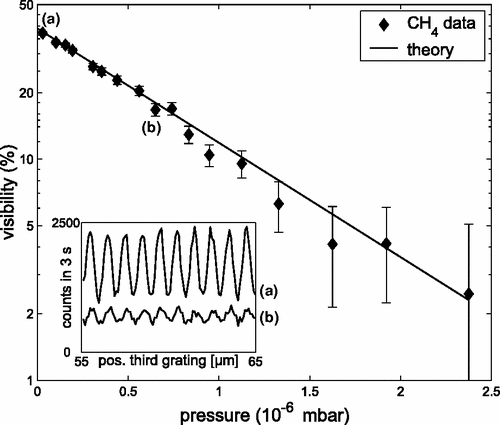
\includegraphics[width=.6\textwidth]{gfx/compton/incoherent-fullerene.png}
    \caption[Visibility of a fullerene interferometer.]{Visibility of the fullerene Talbot-Lau interferometer as a
    function of methane gas pressure. As the pressure is increased, so does
the probability of incoherent scattering of the fullerene molecules with the
molecules of the gas. This exponentially suppresses the visibility of the
interferometer, as shown by the solid line. Reprinted figure with permission
from Hornberger K, Uttenthaler S, Brezger B, Hackerm\"uller L, Arndt M,
Zeilinger A, \emph{Collisional Decoherence Observed in Matter Wave
Interferometry}, Phys. Rev. Lett., 90, 16, 160401, 2003. Copyright 2003 by
the American Physical Society~\parencite{PhysRevLett.90.160401}.}
    \label{fig:incoherent-scattering-fullerene}
\end{figure}

Although in our case we employ photons instead of fullerene molecules, the
same argument holds: incoherent scattering localizes the wave function of
the photon, thus making interference impossible. In the
context of grating interferometry with photons, this would mean that the
dark-field signal would follow the Beer-Lambert law~\ref{eq:beer-lambert}
with an exponential decay for \emph{any} sample, even those that do not
contain microstructures tipically generating such contrast.         

However, one important hypothesis does not hold for the design of our
interferometers, namely:

\begin{quote}
    "[our experiment] is
    based on a Talbot-Lau interferometer with a wide acceptance angle.
    Consequently, a fullerene molecule still enters the detector after a
    typical collision."~\parencite{PhysRevLett.90.160401}
\end{quote}

We can show that this is in fact not the case in our experiments, as a photon typically does
\emph{not} enter the detector after a collision. Consider the sketch in
figure~\ref{fig:sketch-compton}.

\begin{figure}[htb]
    \centering
    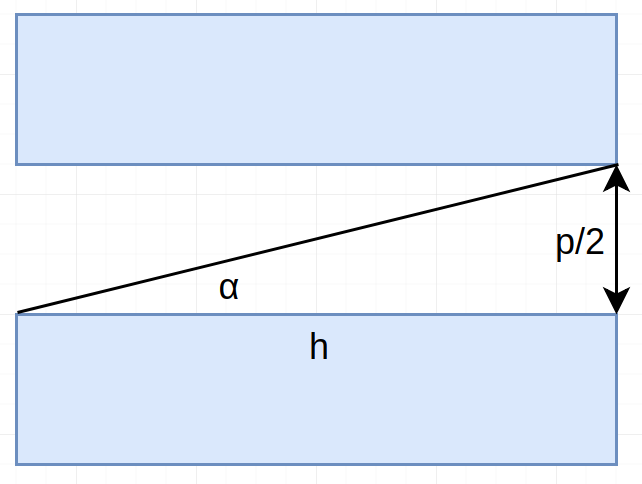
\includegraphics[width=\textwidth]{gfx/compton/compton_deviation.png}
    \caption[X-rays limiting angle after a scattering event.]{Maximum angle
        for the deviation of an X-ray photon after incoherent
    scattering. The photon reaches the detector only if the angle $\alpha$
is small enough that the photon is not subsequently absorbed by the grating.}
    \label{fig:sketch-compton}
\end{figure}

The X-ray photon interacts with the sample, and after incoherent scattering
it is detected only if the angle $\alpha$ is small enough that the grating
does not block it after the interaction. By using the small angle
approximation $\alpha \sim \sin\alpha \sim\tan\alpha$ and the orders of
magnitude of the distances $h \sim \SI{100}{\micro\meter}$ and grating
periods $p \sim \SI{2}{\micro\meter}$ used across all of our
experiments

\begin{equation}
    \alpha < \frac{p}{2h} \simeq
    \frac{\SI{1}{\micro\meter}}{\SI{100}{\micro\meter}} = 10^{-2}
    \label{eq:acceptance-angle}
\end{equation}

Only photons scattered within such a small deviation are detected
incoherently at the detector and contribute to the loss of visibility as
described in~\parencite{PhysRevLett.90.160401}. However, the differential cross
section for the incoherent scattering of photons from electrons can be
approximated with the Klein-Nishina formula~\parencite{Klein1929}

\begin{equation}
    \frac{\de \sigma}{\de \cos \alpha} =
    \frac{\pi\hslash^2\alpha_{fs}^2}{m_e^2c^2}\left(
    \frac{k^\prime}{k} \right)^2 \left( \frac{k}{k^\prime} +
    \frac{k^\prime}{k} - \sin^2 \alpha\right),
    \label{eq:klein-nishina}
\end{equation}

where $\hslash$ is the reduced Planck's constant, $c$ is the speed of light,
$m_e$ is the mass of the electron, $k$ is the momentum of the incident
photon, $k^\prime$ is the momentum of the emitted photon and
$\alpha_{fs} = 1/137$ is the fine structure constant. 
As a consequence of high probability for large scattering angles
(figure~\ref{fig:klein-nishina}) involved in incoherent
scattering, the absorption grating \G2 installed in a Talbot-Lau
interferometer suppresses scattered radiation.

\begin{figure}[htb]
    \centering
    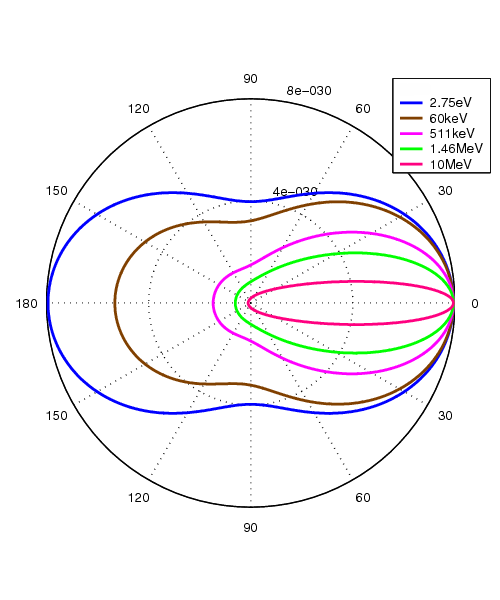
\includegraphics[width=.7\textwidth]{gfx/compton/Klein-Nishina_distribution.png}
    \caption[Klein-Nishina differential cross section.]{Klein-Nishina differential cross
        section~\eqref{eq:klein-nishina}. Reproduced from the public
        domain~\parencite{klein-nishina-plot}.}
    \label{fig:klein-nishina}
\end{figure}

Therefore, after a typical incoherent interaction, a photon does not reach
the detector, hence its contribution to the dark-field signal is suppressed
by a factor of at least 100 but it
is revealed in the transmission signal as absorption by extinction of the
beam. This is also confirmed through Monte Carlo simulations described
in~\cite{silviathesis}. A source spectrum with a gaussian distribution
around \SI{60}{\kilo\eV} for the edge-on interferometer is simulated. In the
Monte Carlo simulation it is possible to follow individual particles and to
track which kind of interaction occurred before hitting the detector.
We can therefore conclude that the influence of Compton scattering on the
dark-field in our experiments (figure~\ref{fig:silvia}) is suppressed
by at least two orders of magnitude by the grating geometry.

\begin{figure}[htb]
    \centering
    \begin{subfigure}[b]{.49\textwidth}
    \centering
    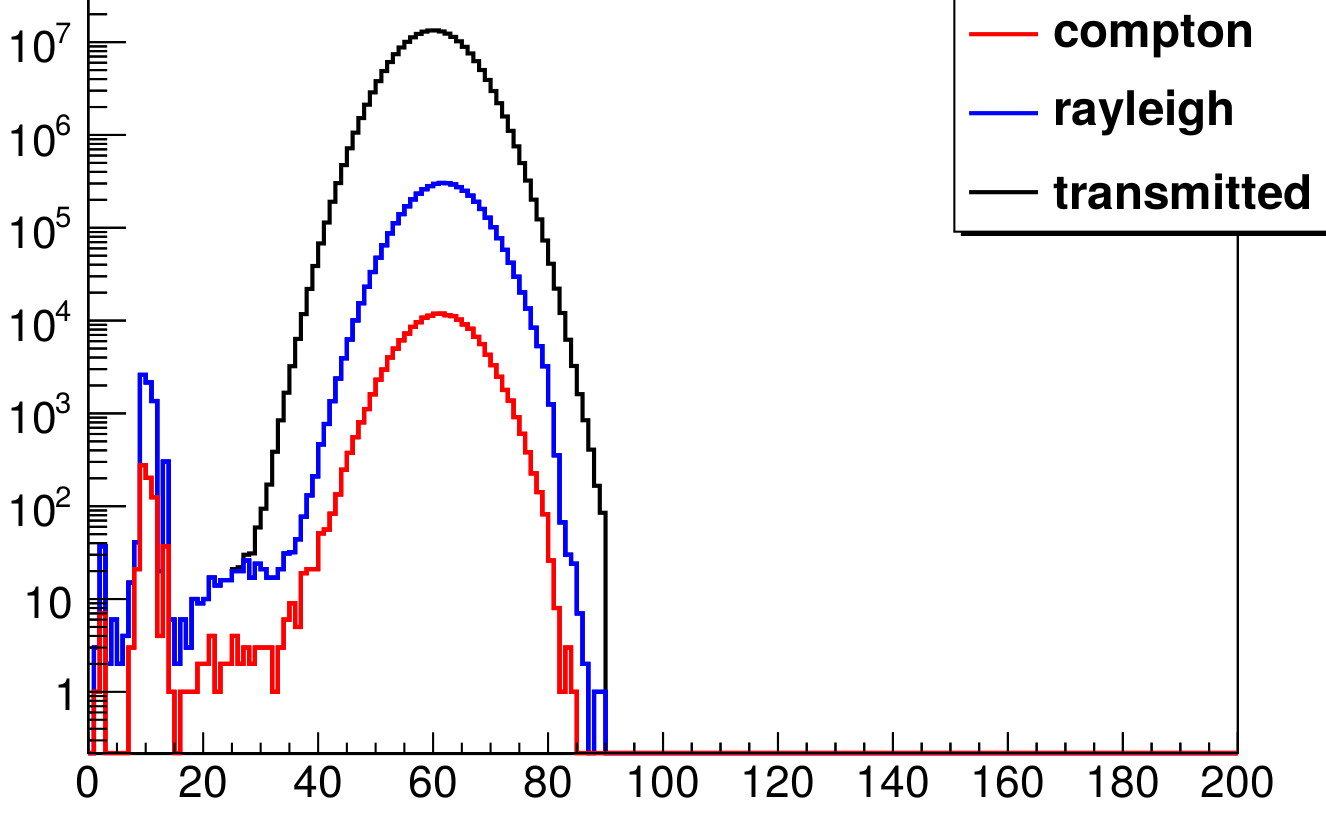
\includegraphics[width=\textwidth]{gfx/compton/scattering_monte_carlo_energy.png}
    \caption{}
    \end{subfigure}
    \begin{subfigure}[b]{.49\textwidth}
    \centering
    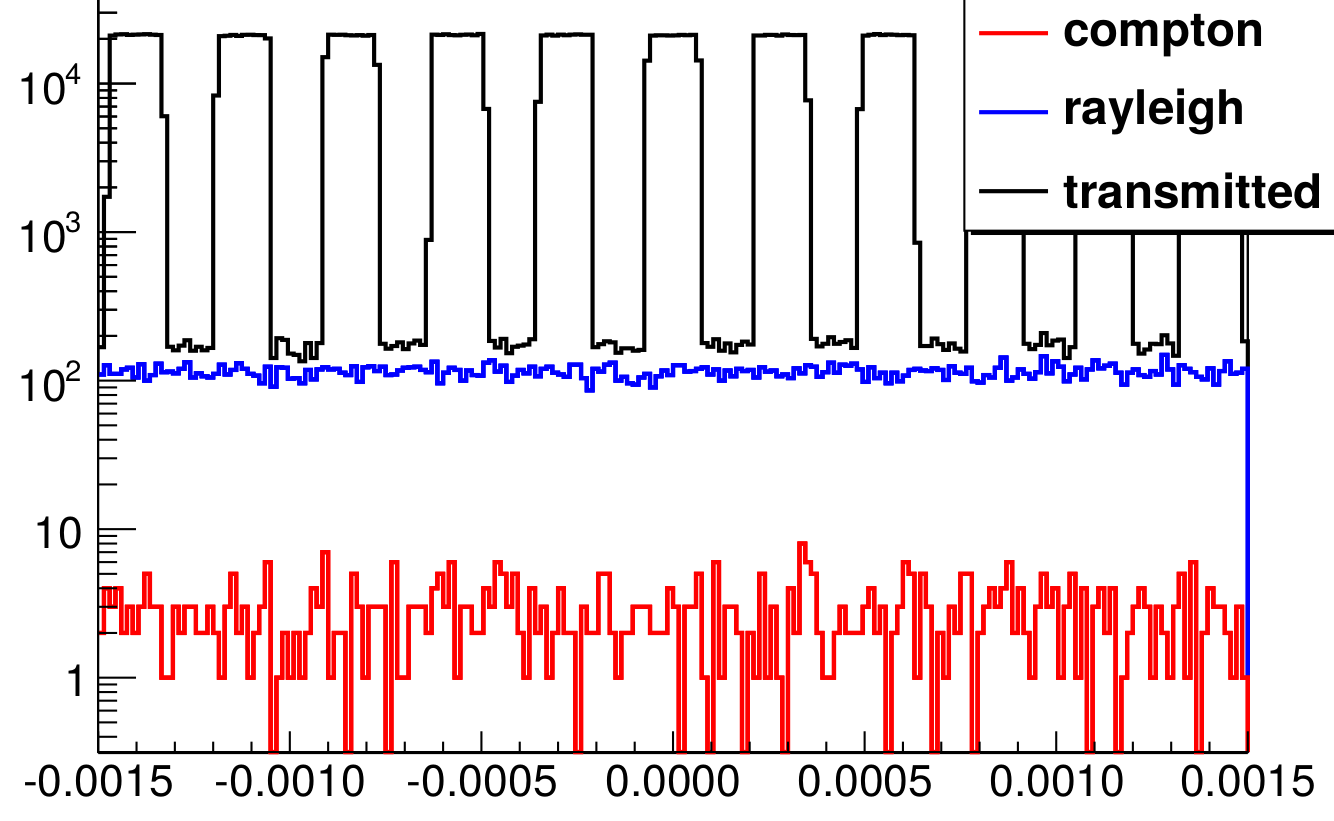
\includegraphics[width=\textwidth]{gfx/compton/scattering_monte_carlo_position.png}
    \caption{}
    \end{subfigure}
    \caption[Monte-Carlo simulation of a grating interferometer.]{The edge-on grating interferometer simulated with the software
        described in~\cite{silviathesis}. The source spectrum as seen from
    the detector on the left, a line profile of the simulated image on the
right, distinguishing the photons by interaction type: the rectangular shape
of the interference pattern can be seen, while Compton scattering is
completely negligible.}
    \label{fig:silvia}
\end{figure}

\section{Conclusion}
In this chapter we described a few technical and scientific issues related
to the operation of high-energy Talbot interferometry setups. We can
conclude, with experiments from the edge-on setup and an improved detector
matching the beam geometry, that quantitative absolute phase sensitivity can
be achieved for elements with a low atomic number, such as plastic phantoms.
Moreover, in order to achieve a quantitative estimation of the
dark-field signal it was necessary to analyze through theoretical and
simulation results the effects of Compton scattering. We were able to
conclude that this effect has a small influence on the dark-field signal,
but it is
detected as absorption contrast through extinction of the beam. Scattering can significantly reduce contrast
in absorption radiography, and antiscatter grids are a known means of
preventing contrast and resolution loss~\parencite{doi:10.1118/1.4811156}. 
In our case, these grids with a high aspect ratio are consituted by the
gratings of the interferometer, which provide for this reason an improvement
in the image quality of the absorption image.
